\documentclass[12pt,letterpaper]{article}

\usepackage{amsmath, amsthm, amsfonts, amssymb}
\usepackage{microtype, parskip, graphicx}
%\usepackage[comma,numbers,sort&compress]{natbib}
\usepackage[style=numeric-comp,
      backend=biber,
      bibencoding=utf8,
      maxbibnames=10,
      uniquename=init,
      giveninits=true,
      sorting=none,
      natbib=true,
      url=false,
      doi=false,
      isbn=false]{biblatex}
\usepackage[margin=1in]{geometry}
\usepackage{lineno}
\usepackage{longtable}
\usepackage{caption, subcaption, multirow, morefloats, rotating}
\usepackage{wrapfig}
\usepackage{hyperref}
\usepackage{threeparttable}

\frenchspacing


\newcommand{\beginsupplement}{
 \setcounter{section}{0}
 \renewcommand{\thesection}{S\arabic{section}}
 \setcounter{table}{0}
 \renewcommand{\thetable}{S\arabic{table}}
 \setcounter{figure}{0}
 \renewcommand{\thefigure}{S\arabic{figure}}
 \setcounter{equation}{0}
 \renewcommand{\theequation}{S\arabic{equation}}
}

% https://3d.bk.tudelft.nl/hledoux/blog/fiddling-biblatex/
%-- formatting hell for biblatex
%-- remove "In:"
\renewbibmacro{in:}{}
%-- no "quotes" around titles of chapters/article titles
\DeclareFieldFormat[article, inbook, incollection, inproceedings, misc, thesis, unpublished]
{title}{#1}
%-- no punctuation after volume
\DeclareFieldFormat[article]{volume}{ {#1} } 
%-- puts number/issue between brackets
\DeclareFieldFormat[article, inbook, incollection, inproceedings, misc, thesis, unpublished]{number}{\mkbibparens{#1}} 
%-- and then for articles directly the pages w/o any "pages" or "pp." 
\DeclareFieldFormat[article]{pages}{#1}
%-- for some types replace "pages" by "p."
\DeclareFieldFormat[inproceedings, incollection, inbook]{pages}{p. #1}

% https://tex.stackexchange.com/questions/81569/biblatex-parentheses-around-the-volume-number-of-an-article
\renewbibmacro*{volume+number+eid}{%
 \printfield{volume}%
 \printfield{number}%
 \printfield{eid}}
\DeclareFieldFormat[article]{number}{\mkbibparens{#1}}


% bibliographic information
%\bibliographystyle{abbrvnat}
%\bibliography{citations}
\addbibresource{citations.bib}






\title{How predictable is extinction? Forecasting species survival at million-year timescales}
\author{
 Smits, Peter\\
 %Department of Integrative Biology, University of California Berkeley\\
 \texttt{psmits@berkeley.edu} 
 \and
 Finnegan, Seth\\
 %Department of Integrative Biology, University of California Berkeley\\
 \texttt{sethf@berkeley.edu}
}
\date{}

\begin{document}

\begin{refsection}

\maketitle

\linenumbers{}
\modulolinenumbers[3]

\begin{abstract}
  A tenet of conservation palaeobiology is that knowledge of past extinction patterns can help us to better predict future extinctions. Although the future is unobservable, we can test the strength of this proposition by asking how well models conditioned on past observations would have predicted subsequent extinction events at different points in the geological past. To answer this question, we analyze the well-sampled fossil record of Cenozoic planktonic microfossil taxa (Foramanifera, Radiolaria, diatoms, and calcareous nanoplankton). We examine how extinction probability varies over time as a function of species age, time of observation, current geographic range, change in geographic range, climate state, and change in climate state. Our models have a 70-80\% probability of correctly forecast the rank order of extinction risk for a random out-of-sample species pair, implying that determinants of extinction have varied only modestly through time. We find that models which include either historical covariates or account for variation in covariate effects over time yield equivalent forecasts, but a model including both is overfit and yields biased forecasts. An important caveat is that human impacts may substantially disrupt range-risk dynamics so that the future will be less predictable than it has been in the past.

\end{abstract}

{\bf Keywords:} conservation, palaeobiology, extinction, forecasting



\section{Introduction}

The intensifying biodiversity crisis confronts conservation biologists with the difficult task of trying to predict which species are most threatened with extinction in the near future. Predicting which species will go extinct is difficult because reliable population and geographic range time series are typically known for only the past few decades in even the best-studied groups, and because few modern extinctions have been adequately documented. This has led to the suggestion that some risk assessments might be improved by incorporating palaeontological data \citep{Finnegan2015,Kiessling2016}. The fossil record preserves information about the full histories, include ultimate extinction, of thousands of lineages, and this information can help to augment the shorter-term higher-resolution data used to make risk assessments of extant taxa.

Extinction intensity (average rate) and selectivity (difference in risk among taxa) have varied greatly through time, and the relative risk of extinction exhibited by different taxonomic and ecological groups can provide insights into the drivers of both background and mass extinction \citep{Payne2007,Payne2016,Ezard2011,Smits2019,Wang2008a,Knoll2007}. Many studies have examined the effects of various potential predictors on extinction risk through time \citep{Harnik2011,Smits2015,Peters2008,Payne2007,Harnik2012,Harnik2012a,Ezard2011,Foote2006} or refined methods for identifying and measuring these effects \citep{Alroy2010a,Alroy2014,Alroy2001,Alroy2000,Alroy2000b,Foote2001}. These studies have produced a growing body of knowledge regarding which factors have been general determinates of extinction risk in the geological past. 

A related question that has received much less attention is how successful we might expect to be when using this knowledge to attempt to predict future extinction events.

Because future extinctions are unobservable we cannot directly evaluate the ultimate performance of such predictions. However, we can take a given point in the geological past, develop a predictive model based on extinction patterns prior to that point, and assessing the predictive performance of this model on subsequent (e.g. ``future'', from the point of view of the model) extinction/survival events. Putting aside the very important question of how human activities will alter the determinants of future extinction risk, such an approach provides a framework for evaluating the expected accuracy of future risk assessments based on past extinction events.

%This variation also raises a question: given that extinction intensity and selectivity change over time, how accurate are our assessments based on past events likely to be when applied to the future? Putting aside the important question of how human activities will alter the determinants of future extinction risk, we can address this uncertainty by specifically including and modeling the temporal variation in extinction risk across a range of extinction intensities and selectivities.

Here we take this approach, using as a model system the Cenozoic record of skeletonized marine planktonic microorganisms (Foraminifera, Radiolaria, diatoms, and calcareous nannoplankton including coccolithophores). This record has several key strengths for our purposes: planktonic microorganisms are widespread and abundant in pelagic habitats, have high preservation potential, and because of their utility for biostratigraphic, paleoclimatic, and oceanographic study they have been the focus of an extensive international coring and study effort \citep{Lazarus1994,SpencerCervato1999}. A compliation of these data is readily available through the Neptune database, an online repository of species occurrences obtained through the Deep Sea Drilling Program and the Ocean Drilling Project \citep{Lazarus1994,SpencerCervato1999}. This database provides abundant samples in space and time, a high degree of temporal resolution for the entirety of the Cenozoic, and has an taxonomic synonymization framework for dealing with 50+ years of taxonomic opinion \citep{Lazarus1994} -- as close to ideal data for this analysis as possible. Analyzing patterns of extinction and global occurrence at fine temporal scales means we can better elucidate how well we can predict species extinction at human-relevant scales.


The overall question of how well models based on past extinction patterns perform at forecasting future extinctions depends in part on model complexity. Simple models requiring only a few parameters are in general preferable because more complex models run a greater risk of being overfit to the observations on which they are trained. In addition, many traits that might influence extinction risk among extant species are difficult to assign confidently to extinct species. For these reasons we elect to focus on “baseline” models which include only a few parameters that have been shown to be important and/or consistent determinants of extinction risk in the marine fossil record. Numerous studies have established that geographic range is one of the most important determinants of extinction risk in the fossil record, and that a species’ geographic range can be highly variable over geologic time \citep{Foote2007,Liow2010,Liow2007,Kiessling2013,Payne2007,Jablonski2003,Jablonski2008,Jablonski2006}. In addition to geographic range, we also considered global climate state and change in climate state since previous observation in order to evaluate the influence of climate or climate change trajectory on extinction risk. Finally, we included species age, both because previous studies of planktonic taxa have found it to be a determinant of extinction risk and because its inclusion in our models is critical to their nature as survival models (see Model Specifications below). We reiterate that our primary objective is to evaluate the predictive performance of simple models that include only a few general parameters; more complex models including other likely determinants of extinction risk such as skeletal mineralogy, trophic ecology, and thermal tolerance range might well perform better.



There are a number of ways in which past extinction patterns might be used to model present risk. The simplest case assumes that relationships between predictors (hereafter covariates) and extinction risk have been constant through time. A more complex but more realistic case allows relationships between covariates and extinction risk to vary through time, consistent with evidence for temporal variation in extinction selectivity regime. Finally, an important consideration is the degree to which species’ geographic range trajectories exhibit deterministic versus Markovian behavior \citep{Liow2007,Kiessling2013,Foote2007b,Pigot2012}. In the former case, knowledge of the specific past trajectory of a species – whether its range has expanded or contracted from some point in the past to the present – might help to improve assessments of its current risk. In the latter case only the current geographic range of the species would convey useful information about current and future risk (although that assessment would still be based on the relative extinction risk of species that had similar ranges at different points in the geological past). In all cases, we use information about the past to predict the future, the question is wheter and how much historical information (e.g. the histories of species over time) improves our ability to forecast future extinction events.

Below, we evaluate four models along a spectrum from simplest (fixed covariate effects, Markovian range dynamics) to most complex (varying covariate effects, deterministic range dynamics). We ask (1) how well they perform at classifying species as extinctions or survivors in the data they were fit to, and (2) how well they perform at classifying species as extinctions or survivors in “future” data that were not used in fitting the models.



\section{Materials and Methods}

\subsection{Data Specifications}

We analyzed microfossil occurrence information from the Neptune Database \url{http://www.nsb-mfn-berlin.de/nannotax} \citep{Lazarus1994,SpencerCervato1999}. This occurrence-based dataset includes calcareous nannoplankton, diatoms, planktonic Foraminifera, and radiolarians. Occurrences were filtered to include only those species with first occurrences no earlier than 63 Mya (millions of years ago). This filtering criterion excludes taxa that survived the K/Pg extinction or arose during this recovery interval, and ensures that our occurrence histories fully overlap with the temperature time-series used as a potential extinction risk predictor (see below). 

All fossil occurrences were assigned to 1 My (million year) bins based on the estimated age of the fossil occurrence as listed in the Neptune Database. After binning, each species' geographic range was calculated for each of the 1 My bins in which it occurred. Geographic range was calculated as the minimum spanning tree distance between all observations of that taxon during that temporal bin; this distance was measured in kilometers. Minimum spanning tree distance was calculated using the \texttt{GeoRange} package for R \citep{GeoRange}. 

We also included how a taxon's geographic range has changed since its last three observation times. We measured this change in geographic range by calculating the difference in geographic range between an observation and that taxon's three previous occurrences. Change between the most recent and the three previous occurrences was calculated individually for each of those lags. If there are not enough previous observations to calculate, then that value is recorded as a 0. These differences were calculated after minimum spanning tree distance was transformed and standardized (see Supplement Section S1.1.2)

Average global temperature of each 1 My bin was calculated from estimates based on Magnesium/Calcium isotope ratios \citet{Cramer2011}. We use Mg/Ca rather than oxygen isotopes to avoid confounding effect of varying ice-volume -- this property is of particular importance for this analysis as polar ice-caps develop midway through the Cenozoic. Estimating temperature over long periods of time from Mg/Ca ratios also suffers from complications because Mg/Ca based temperature estimates requires benthic Foraminifera and seawater Mg/Ca isotope ratio information. Because seawater Mg/Ca ratio has changed over time, the method to estimate temperature used \citet{Cramer2011} attempts to account for this unknown in order to obtain accurate, albeit uncertain, temperature estimates. Our data source, \citet{Cramer2011}, estimated temperature for every 0.1 My interval between 0 to 63 Mya. The temperature estimate for each 1 My interval was calculated as the mean of all estimates within that interval. 

We also included the global temperature from the previous time that taxon was observed. If there are not enough previous observations to calculate, then that value is recorded as a 0. This lag was calculated after global temperature was transformed and standardized (see Supplement Section S1.1.2).

Mg/Ca based temperature estimates are measured from benthic Foraminifera, and are an estimate of deep water ocean temperature. The organisms in this study are all planktonic, Mg/Ca based temperature estimates do not describe the exact environment these organisms inhabit. Ideally, we would have detailed ocean surface water temperature estimates for the entire globe for the entire Cenozoic. Unfortunately, that type of data does not exist. So, we interpret our temperature estimates as reflecting the global climate state that an organisms experiences, and not as a descriptor of that taxon's local environmental ecology.

See Supplemental Section S1.1 for a further explanation on how observations were temporally binned, and how our covariates were standardized and transformed prior to analysis.


%\begin{figure}[ht]
% \centering
% 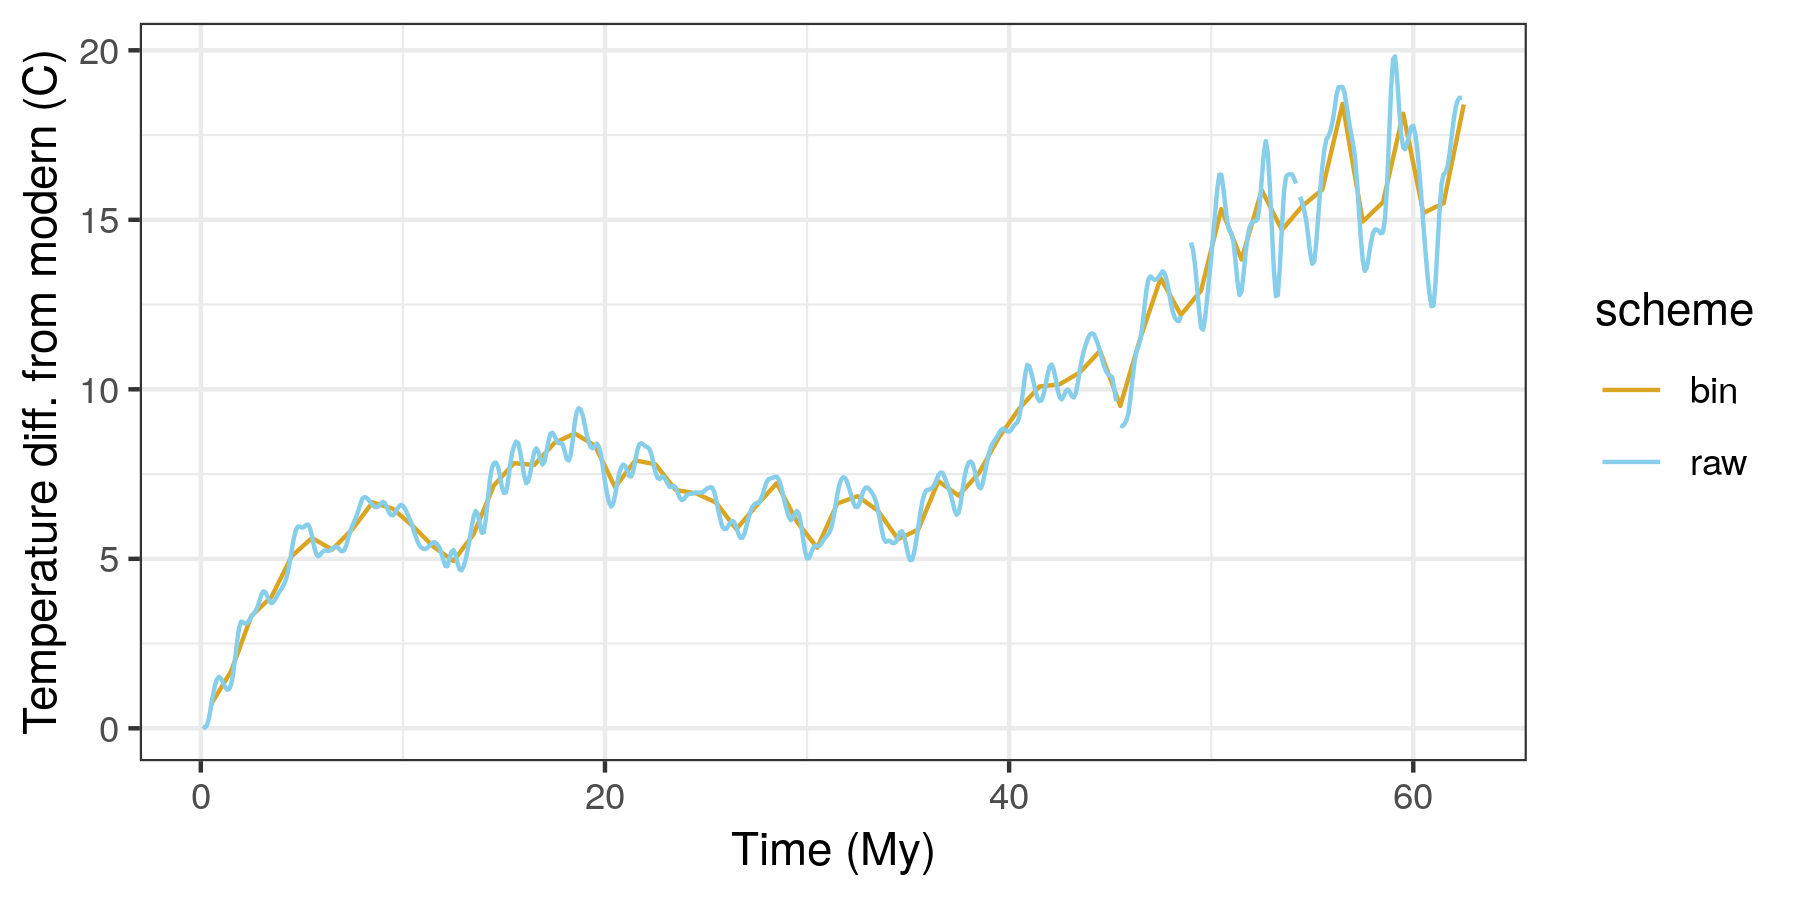
\includegraphics[width=\textwidth,height=0.5\textheight,keepaspectratio=true]{../results/figure/cramer_temp}
% \caption{Comparison of initial temperature estimates from \citet{Cramer2011} (goldenrod) versus the binned values used in this analysis (blue). The initial values are for every 0.1 My while our bins are defined for every 1 My.}
% \label{fig:temp_curve}
%\end{figure}


\subsection{Model Specifications}

We used a discrete-time survival modelling framework to estimate how well we can predict extinction risk at one million year time scales. At its core, our model is a multilevel logistic regression with taxon age in millions of years as a varying intercept \citep{Tutz2016}. We considered four different models involving different permutations of covariate effects (fixed or time-varying) and historical covariates: covariate effects constant over time and no historical covariates included (Model C), covariate effects allowed to vary over time but no historical covariates included (Model V), covariate effects constant over time and historical covariates included (Model CP), and covariate effects allowed to vary over time and historical covariates are included (Model VP). The C and P models attempt to predict based only on present state, whereas the CP and VP models allow for the possibility of non-Markovian behaviour by including change in state from the previous time increment.

We always included species age at time of observation (i.e. observed prior duration) as a varying-intercept term. This factor may or may not contribute to differences in species extinction risk over time \citep{Smits2015,Finnegan2008,Ezard2012,VanValen1973,Liow2011,Crampton2016}, but its inclusion in our model is critical to its nature as a survival model \cite{Tutz2016}. The effect of species age is allowed to vary by taxonomic group. 

Similarly, we included time of obseration as an additional varying-intercept term to account for changes average global extinction risk over time that are not related to the covariates included in this model. This varying-intercept is further allowed to vary by taxonomic group. This varying-intercept term allows us to tease apart the differences in extinction risk associated with time of observation versus age since first observation. An important note is that for our V and VP models, the covariation between this varying-intercept and the varying-slopes of our covariates is explicitly modeled (see Supplement Section S1.2).

See Table \ref{tab:model_def} for further explanation of how the four models we considered differ from each other. A complete description of the statistical model used in this analysis is available in Supplement Section S1.2. Additionally, the full description of how these models were implemented and coded, including choice of priors, is available in Supplement Section S1.2.


\begin{table}[ht]
 \caption{Models and their definitions}
 \begin{threeparttable}
  {
   \def\arraystretch{1.5}
   \begin{tabular}{ l p{3cm} l l }
    Code & Description & Covariates & R Formula Syntax\tnote{a}\phantom{\textsuperscript{a}} \\
    \hline
    C & Constant effects, no historical cov. & \parbox[t]{0.25\textwidth}{Geographic range,\\temperature} & \parbox[t]{0.33\textwidth}{event\tnote{b}\phantom{\textsuperscript{b}} $\sim$ range\tnote{c}\phantom{\textsuperscript{c}} + temp\tnote{d}\phantom{\textsuperscript{d}} +\\(1 $|$ time\tnote{e}\phantom{\textsuperscript{e}}/phylum\tnote{f}\phantom{\textsuperscript{f}}) +\\(1 $|$ age\tnote{g}\phantom{\textsuperscript{g}}/phylum)} \\
    V & Varying effects, no historical cov. & \parbox[t]{0.25\textwidth}{Geographic range,\\temperature} & \parbox[t]{0.33\textwidth}{event $\sim$ range + temp +\\(1 + range + temp $|$ time/phylum) + (1 $|$ age/phylum)} \\ 
    CP & Constant effects, historical cov. & \parbox[t]{0.25\textwidth}{Geographic range,\\change in geographic range, temperature,\\previous temperature} & \parbox[t]{0.33\textwidth}{event $\sim$ + range\_diff1\tnote{g}\phantom{\textsuperscript{h}} + range\_diff2\tnote{h}\phantom{\textsuperscript{h}} + range\_diff3\tnote{h}\phantom{\textsuperscript{h}} + \\temp + temp\_lag\tnote{i}\phantom{\textsuperscript{i}} +\\(1 $|$ time/phylum) +\\(1 $|$ age/phylum)} \\
    VP & Varying effects, historical cov. & \parbox[t]{0.25\textwidth}{Geographic range,\\change in geographic range, temperature,\\previous temperature} & \parbox[t]{0.33\textwidth}{event $\sim$ range + range\_diff1 + range\_diff2 + range\_diff3 + \\temp + temp\_lag +\\(1 + range + range\_diff1 + range\_diff2 + range\_diff3 +\\temp + temp\_lag $|$ time/phylum) +\\(1 $|$ age/phylum)} \\
    \hline
   \end{tabular}
  }
  \begin{tablenotes}
  \item[a] See Supplemental Equation S2 for full statistical model definition.
  \item[b] Species observation where 1 if time of last observation, otherwise 0.
  \item[c] Species geographic range in log km\(^2\). Mean centered, scaled to sd = 1.
  \item[d] Global temperature in degrees C. Mean centered, scaled to sd = 1.
  \item[e] Time of observation.
  \item[f] Taxonomic group of species (i.e. Foraminifera, diatoms, Radiolaria, calcareous nannoplankton).
  \item[g] Age at observation.
  \item[h] Change in geographic range since last observation (number indicates how lags).
  \item[i] Temperature at previous observation.
  \end{tablenotes}
 \end{threeparttable}
 \label{tab:model_def}
\end{table}


\subsection{In-sample and out-of-sample forecasting}

We are interested in model performance (i.e. forecasting) in two distinct contexts: in-sample performance, and out-of-sample predictive performance.

In-sample forecasting is a posterior predictive check in that we are estimating our model's ability to correctly classify the data to which it was fit. Posterior predictive checks are a type of sensitivity analysis because we are checking the quality of model's fit to the data. If our models have poor in-sample forecasting performance, than our models are not adequate descriptors of the data and will most likely make poor out-of-sample predictions. In-sample forecasting measures, however, are not the same as understanding our models' ability to forecast future extinctions or if our models are overfit to our data and produce biased out-of-sample estimates \citep{ESL}. 

We are particularly interested in understanding how well our model forecasts extinction probability of data from the future that the model was not fit to (out-of-sample data). To quantify our ability to forecast species' extinction risk, we estimated average out-of-sample forecasting performance using 5-fold time-series cross-validation. For time-series data, the folds (data partitions) are approximately equal segments of time. Each fold represents a sequence of time points. With 63 time points, each of the five folds represents approximately 13 million-year time increments. It is important to bear in mind, however, that each time increment includes many (100s-1000s) individual observations.

\textit{k}-fold cross-validation for time series follows a specific sequence of procedures \citep{Arlot2010,Bergmeir2016,ESL}. Prior to cross-valdiation, the data is divided into \textit{k} nearly even segments or folds -- for a time series, this means the data is divided into \textit{k} continuous sequences. Next, the model is fit to the first fold (time segment), and the posterior estimates of that fit are then used to forecast the extinction probability of the second fold (i.e. the future). Then the model is fit to the combined first and second folds, and the posterior estimates of that fit are used to forecast the extinction probability of the third fold. Continuing, the model is then fit to the first three folds combined and is then used to forecast extinction probabilities for the fourth fold. Next, the model is fit to the first four folds combined and then is used to forecast the fifth fold. This process continues until $k - 1$ folds are included in the fitting the model and the final fold is predicted from this model. When combined, the results from these forecasts are then combined to yield our estimate of expected out-of-sample performance. In 5-fold cross validaition, the data is divided into five folds the cross-validation procedure yields predictions for four of the folds.

Cross-validation is a procedure for estimating a model's expected out-of-sample error. Information criteria such as AIC or WAIC are approximations of out-of-sample predictive error as estimated by cross-validation \citep{ESL,Gelman2013d}. Cross-validation implicitly takes into account model complexity because when a model is overfit to its data, out-of-sample predictions will be biased and inaccurate \citep{ESL}. A high degree of similarity between out-of-sample and in-sample estimates indicates that the model is not overfit to the data (though it is not necessarily an adequate descriptor of the data). Cross-validation is preferable to simple metrics such as AIC because instead of a single value it produces an entire posterior distribution of estimates.

The relative adequacy of the four model variants was compared using the area under the receiver operating characteristic curve or AUC \citep{Fawcett2006,Mason2002}. This measure is commonly used to measure the performance of classification models as it has the desirable characteristic of comparing the model's true positive rate with its false positive rate, as opposed to accuracy which only considers true positives. AUC ranges between 0.5 and 1, with 0.5 indicating no difference in classification from random and 1 indicating perfect classification. AUC can be interpreted as the probability that our model correctly ranks the relative extinction risks of a randomly selected extinct-extant species pair \citep{Fawcett2006,Mason2002}. AUC values of approximately 0.8 or greater can be considered ``good'' \citep{ACCDA}, so we consider values between between 0.7 and 0.8 as ``fair,'' and values between 0.6 and 0.7 as ``poor.''

%The differences in in-sample predictive performance between the models was visualized in multiple ways: whole data set by model, taxonomic group by model, model performance over time, and model performance by taxonomic groups over time. These comparisons demonstrate the relative and absolute adequacy of the models in describing the dataset they were fit to.

To reiterate, the primary focus of this study is on understanding how well our models forecast future extinction events by comparing our in-sample and out-of-sample forecast estimates. A presentation of the posterior estimates for the regression coefficient estimates from our VP model (Table \ref{tab:model_def}) is available our Supplemental Materials (Section S2).

See our code repository at https://github.com/psmits/trident for full code details. The entire analysis was coded in R and uses tidyverse and tidyverse adjacent tools such as \texttt{dplyr} \citep{dplyr}, \texttt{purr} \citep{purrr}, and \texttt{tidybayes} \citep{tidybayes}. All of our models were written using the \texttt{brms} \citep{brms2017,brms2018} R package, which implements Stan-based Bayesian models which are fit via Hamiltonian Monte Carlo \citep{StanManual}.


\section{Results}


% ROC model comparison
\begin{figure}[ht]
 \begin{subfigure}[ht]{0.45\textwidth}
   %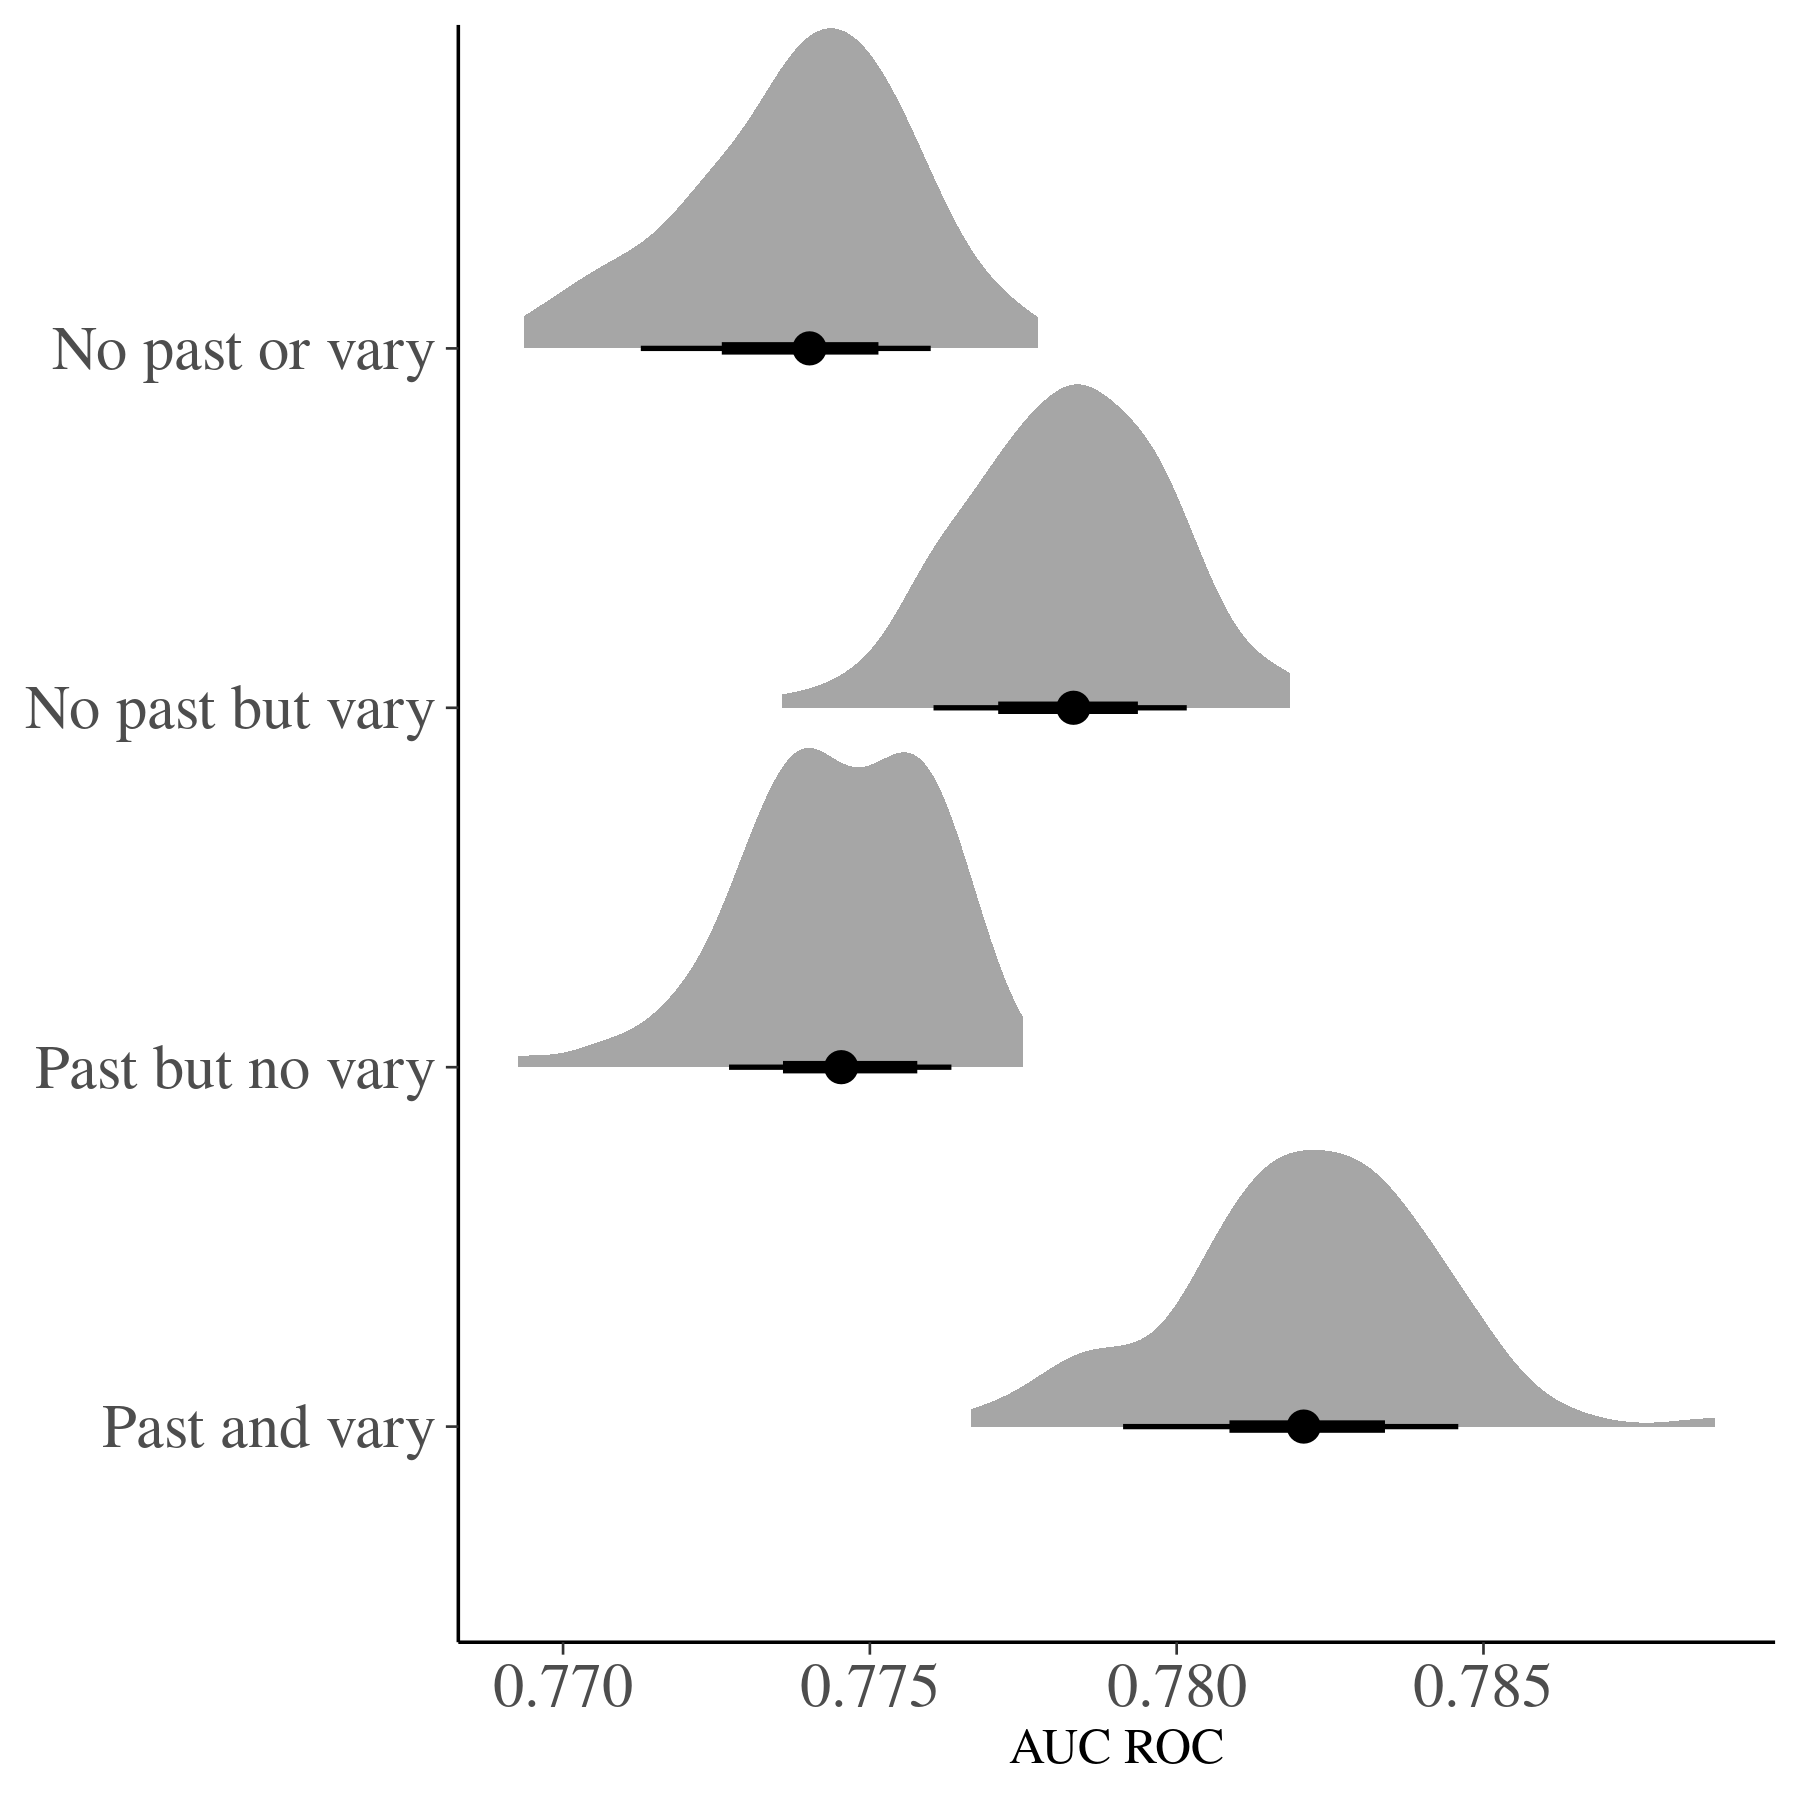
\includegraphics[width=\textwidth,height=0.5\textheight,keepaspectratio=true]{auc_hist_full.png}
  \caption{In-sample}
  \label{fig:auc_hist}
 \end{subfigure}
 \begin{subfigure}[ht]{0.45\textwidth}
   %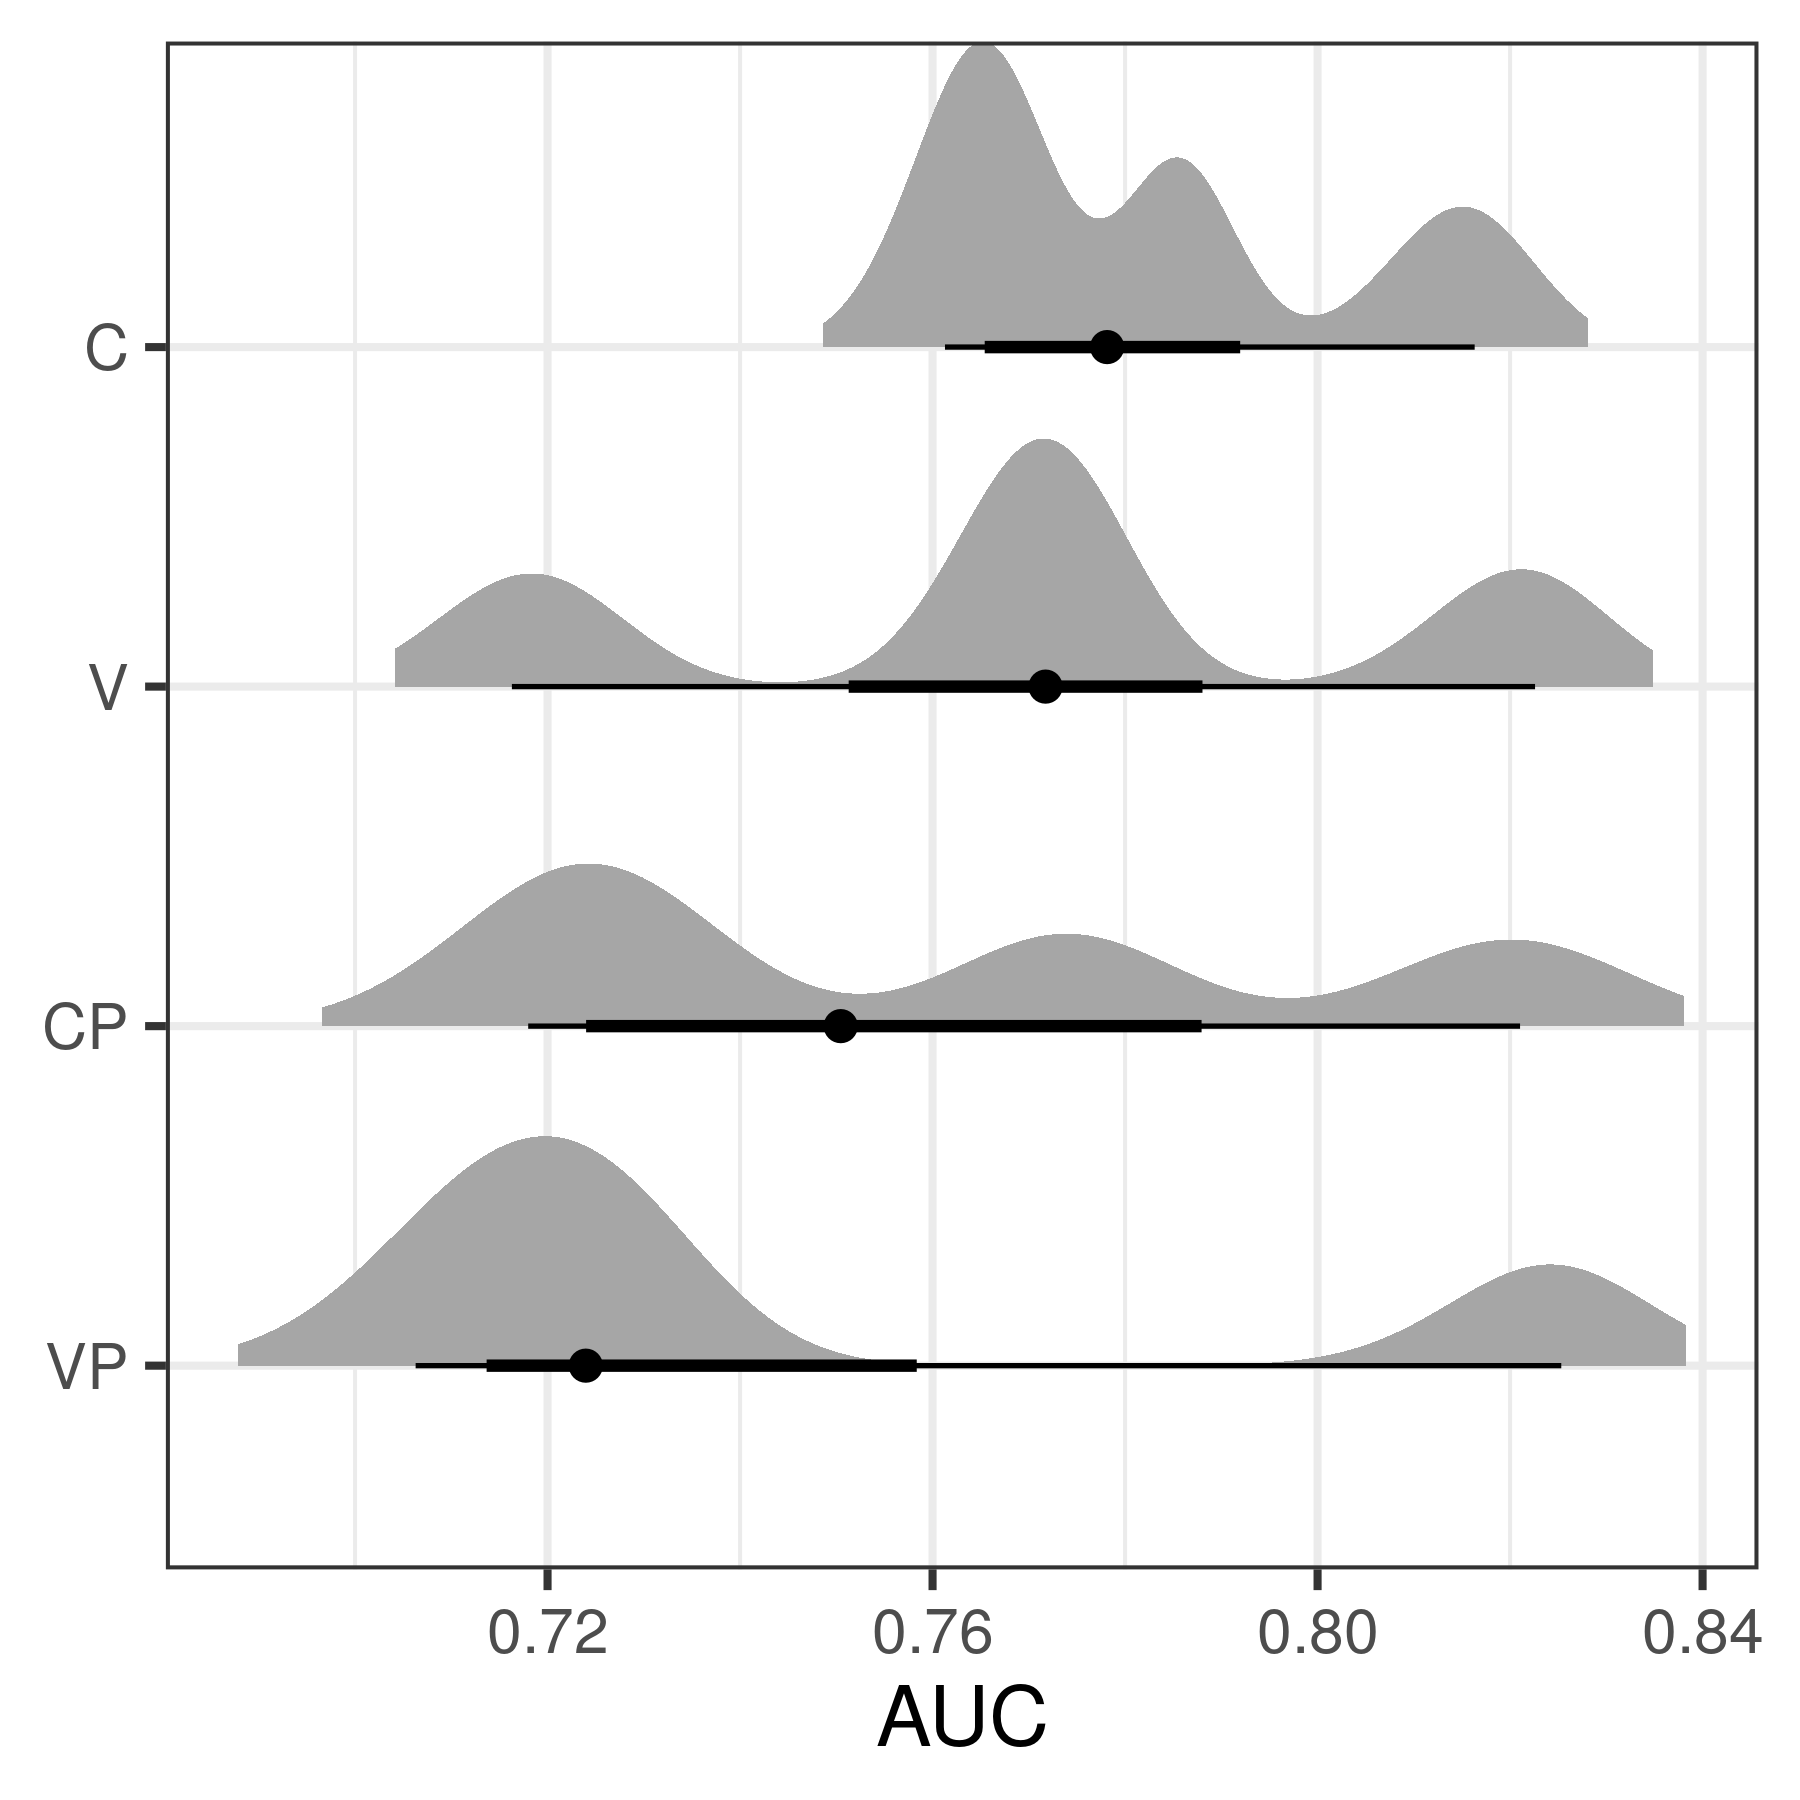
\includegraphics[width=\textwidth,height=0.5\textheight,keepaspectratio=true]{fold_auc_full.png}
  \caption{Out-of-sample}
  \label{fig:fold_auc}
 \end{subfigure}
 \caption{Comparisons of measures of model performance for both in-sample (\ref{fig:auc_hist}) and out-of-sample (\ref{fig:fold_auc}) cross-validation. The area under the receiver operating charactered curve (AUC) was calculated for each model. these estimates are calculated from the models posterior predictive distribution (\ref{fig:auc_hist}) or from predictions made to new data (\ref{fig:fold_auc}), respectively. Marked below the posterior distributions are the median AUC and 50\% and 80\% posterior intervals for all observations in the dataset. Models with higher AUC values indicate better performance over models with lower AUC values. AUC is bounded between 0.5 and 1. See Table \ref{tab:model_def} for an explanation of the four models (C, V, CP, VP).}
 \label{fig:auc_compare}
\end{figure}

\subsection{In-sample forecasting adequacy}

Comparison between the posterior distributions of in-sample AUC for each of the four models demonstrates that the parameter rich model VP has the greatest median in-sample AUC when compared to the other three models, while there is substantial overlap in the posterior distributions of the forecasts from the other three models (Fig. \ref{fig:auc_hist}). 

However, the actual difference in forecast AUC result between the VP model and the other three models is extremely small (0.01 AUC unit), and all of the in-sample AUC estimates from our models are concentrated between an AUC value of 0.775 and 0.795 (Fig. \ref{fig:auc_hist}). This result indicates that the practical difference in performance between these models might be so small that there is no practical benefit that the VP model over the other three. Ultimately, determining which of these models produces the best forecasts of future extinctions requires comparing these in-sample results to our out-of-sample results (see below).

In-sample forecasts from the four models over time are broadly similar among taxonomic groups (Fig. \ref{fig:auc_taxon_time}). In-sample forecasts for diatoms are the weakest of the four taxonomic groups as all four models have several intervals with no predictive power (AUC not significantly greater than 0.5). The best in-sample forecast results are for radiolarians, for which all models have at most 1 interval with little predictive power. The pattern of high and low in-sample forecast performance is broadly similar among the four models.

\begin{figure}[ht]
 \centering
 %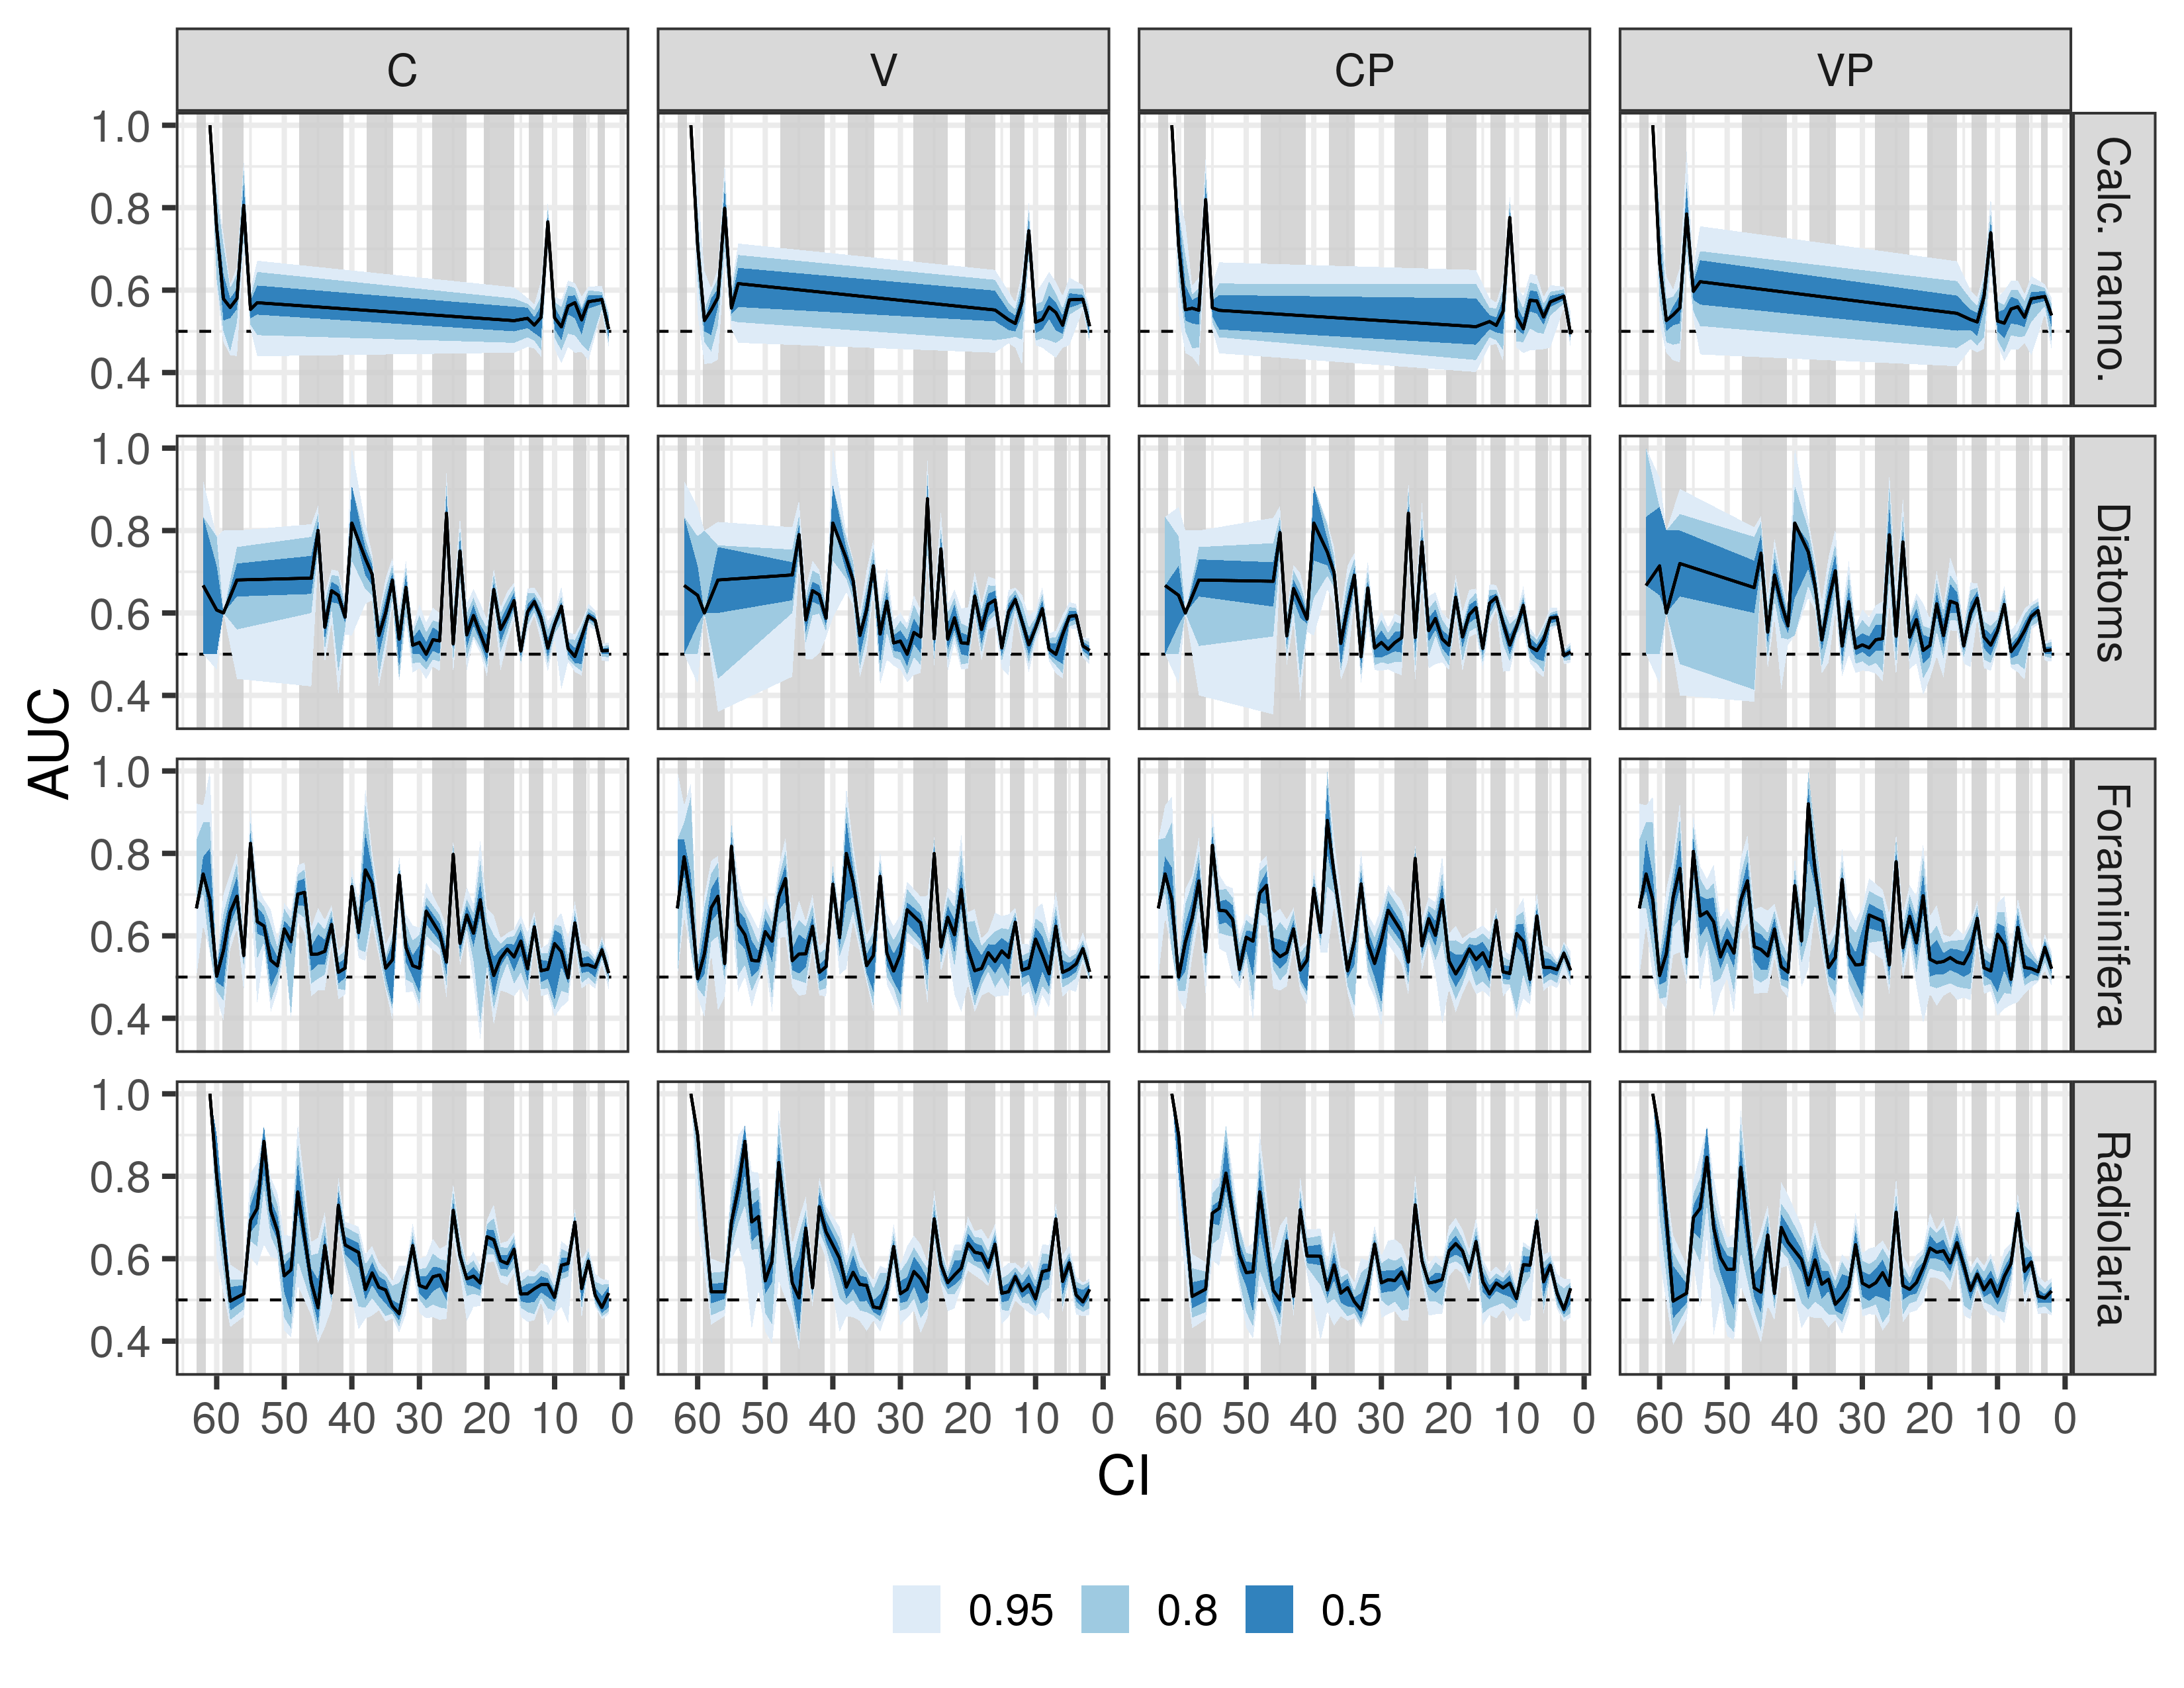
\includegraphics[width=\textwidth,height=0.5\textheight,keepaspectratio=true]{auc_taxon_time_full.png}
 \caption{Understanding model adequacy over time and taxonomic group by comparing in-sample forecasting performance measured by AUC for each of the four models. These estimates reflect each model's fit to the various taxonomic groups over time. The black line corresponds to the median AUC value, while the envelopes correspond to multiple credible intervals as indicated in the legend. In all cases, higher AUC values indicate greater predictive performance versus lower AUC values. The grey intervals mark the geologic ages of the Cenozoic. See Table \ref{tab:model_def} for a description of each of the four models (C, V, CP, VP).}
 \label{fig:auc_taxon_time}
\end{figure}




\subsection{Out-of-sample forecasting performance}

Out-of-sample forecast AUC estimates, based on five-fold cross validation \citep{Arlot2010,Bergmeir2016}, exhibit a broader range than in-sample estimates, with AUC ranging between approximately 0.7 and 0.85 (Fig. \ref{fig:auc_hist}, \ref{fig:fold_auc}). While the VP model has the best in-sample forecasting performance (Fig. \ref{fig:auc_hist}) this model performs poorly at out-of-sample forecasting compared to the other models (Fig. \ref{fig:fold_auc}). The poor out-of-sample performance suggests that this most complex model is overfit and that one of the simpler models would be preferable for predicting future extinctions. Thus the models that include both historical covariates (e.g. change in geographic range) and time-varying effects produce biased extinction forecasts. Interestingly, models that include either historical covariates but assume constant effects (CP) or do not include historical covariates but include time-varying effects (V) perform similarly when forecasting future extinction events (Fig. \ref{fig:auc_compare}). 


As noted above, there were some time intervals in which in-sample forecasts were no better than random (Fig. \ref{fig:auc_taxon_time}). Such intervals are generally much rarer for out-of-sample forecasts. The major exception to this pattern are diatoms, which have at least one time interval for all four models in which the median AUC of the out-of-sample forecasts were no better random. The only other group for which median posterior predictive estimate of out-of-sample AUC reaches 0.5 is calcareous nannoplankton, and then only with the V model.
\begin{figure}[ht]
 \centering
 %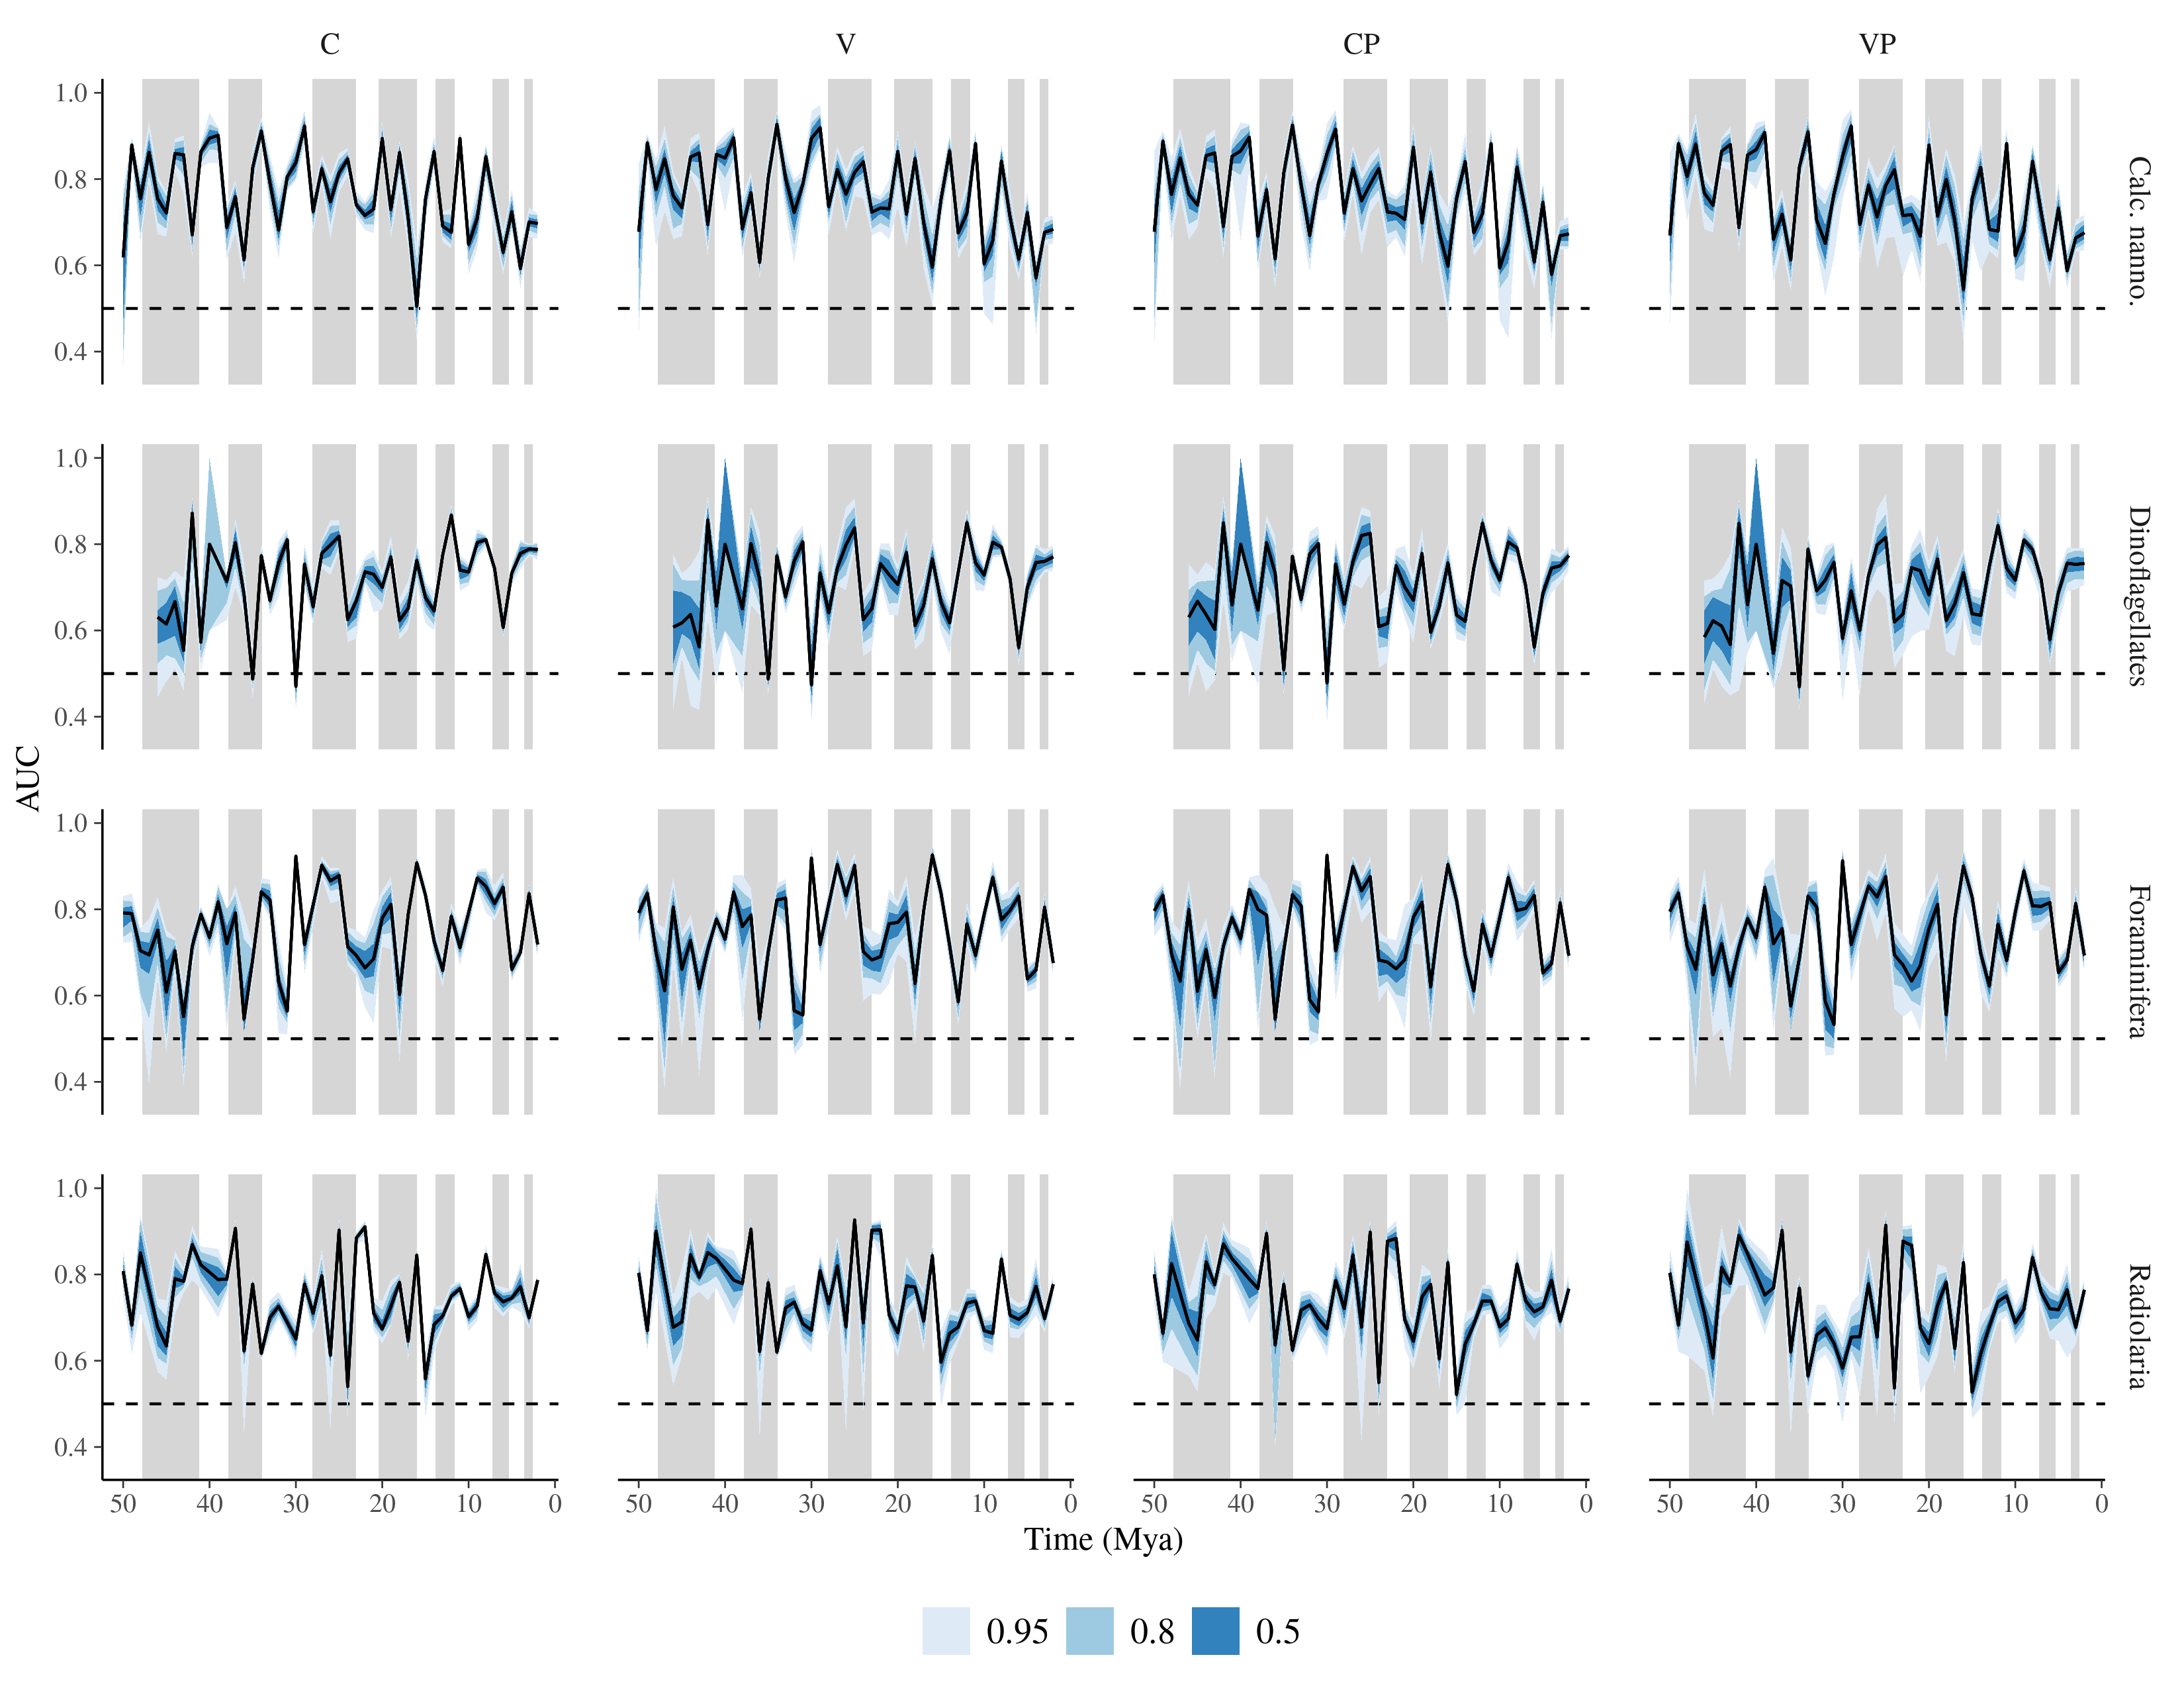
\includegraphics[width=\textwidth,height=0.5\textheight,keepaspectratio=true]{fold_auc_taxon_time_full.png}
 \caption{Comparison of the four models' ability to forecast future extinction events as measured by out-of-sample AUC values over time as aggregated by taxonomic group for each of the four models. The AUC of the individual My intervals within each fold is plotted to highlight the heterogeneity in performance within and between folds. This presentation decomposes each of the 12-million year folds by each of the taxonomic groups into the predictions made for each of the million-year intervals. The black line corresponds to the median AUC estimate, with the envelopes corresponding to multiple credible intervals as indicated in the legend. The grey intervals mark the geologic ages of the Cenozoic. See Table \ref{tab:model_def} for a description of each of the four models (C, V, CP, VP).}
 \label{fig:fold_auc_taxon_time}
\end{figure}

We compared the difference in AUC estimates from the out-of-sample forecasts to the AUC estimates from in-sample forecasts by subtracting the in-sample AUC estimates from the out-of-sample AUC estimates (Fig. \ref{fig:oos_ins_diff}); a difference in AUC close to 0 indicates complete congruence between the in-sample and out-of-sample forecasts. A positive difference indicates that out-of-sample forecasts actually outperform in-sample forecasts, whereas negative difference indicates poorer out-of-sample performance than in-sample forecast. Divergences between out-of-sample and in-sample forecasts are rare and tend not to cluster in time, consistent with the broad visual congruence between the in-sample and out-of-sample performance (Fig. \ref{fig:auc_taxon_time}, \ref{fig:fold_auc_taxon_time}). An example multimillion year pattern indicating significantly poorer out-of-sample forecast performance than in-sample forecast performance is for Radiolaria based on the VP model between 35 Mya and approximately 28 Mya (Fig. \ref{fig:oos_ins_diff}). There exist similar periods of worse out-of-sample forecasting performance for other combinations of taxonomic group and predictive model, for example the CP model has worse out-of-sample forecasting than in-sample for the last 5 million years of the Cenozoic. In general, however, most out-of-sample and in-sample forecasts are almost identical.

\begin{figure}[ht]
 \centering
 %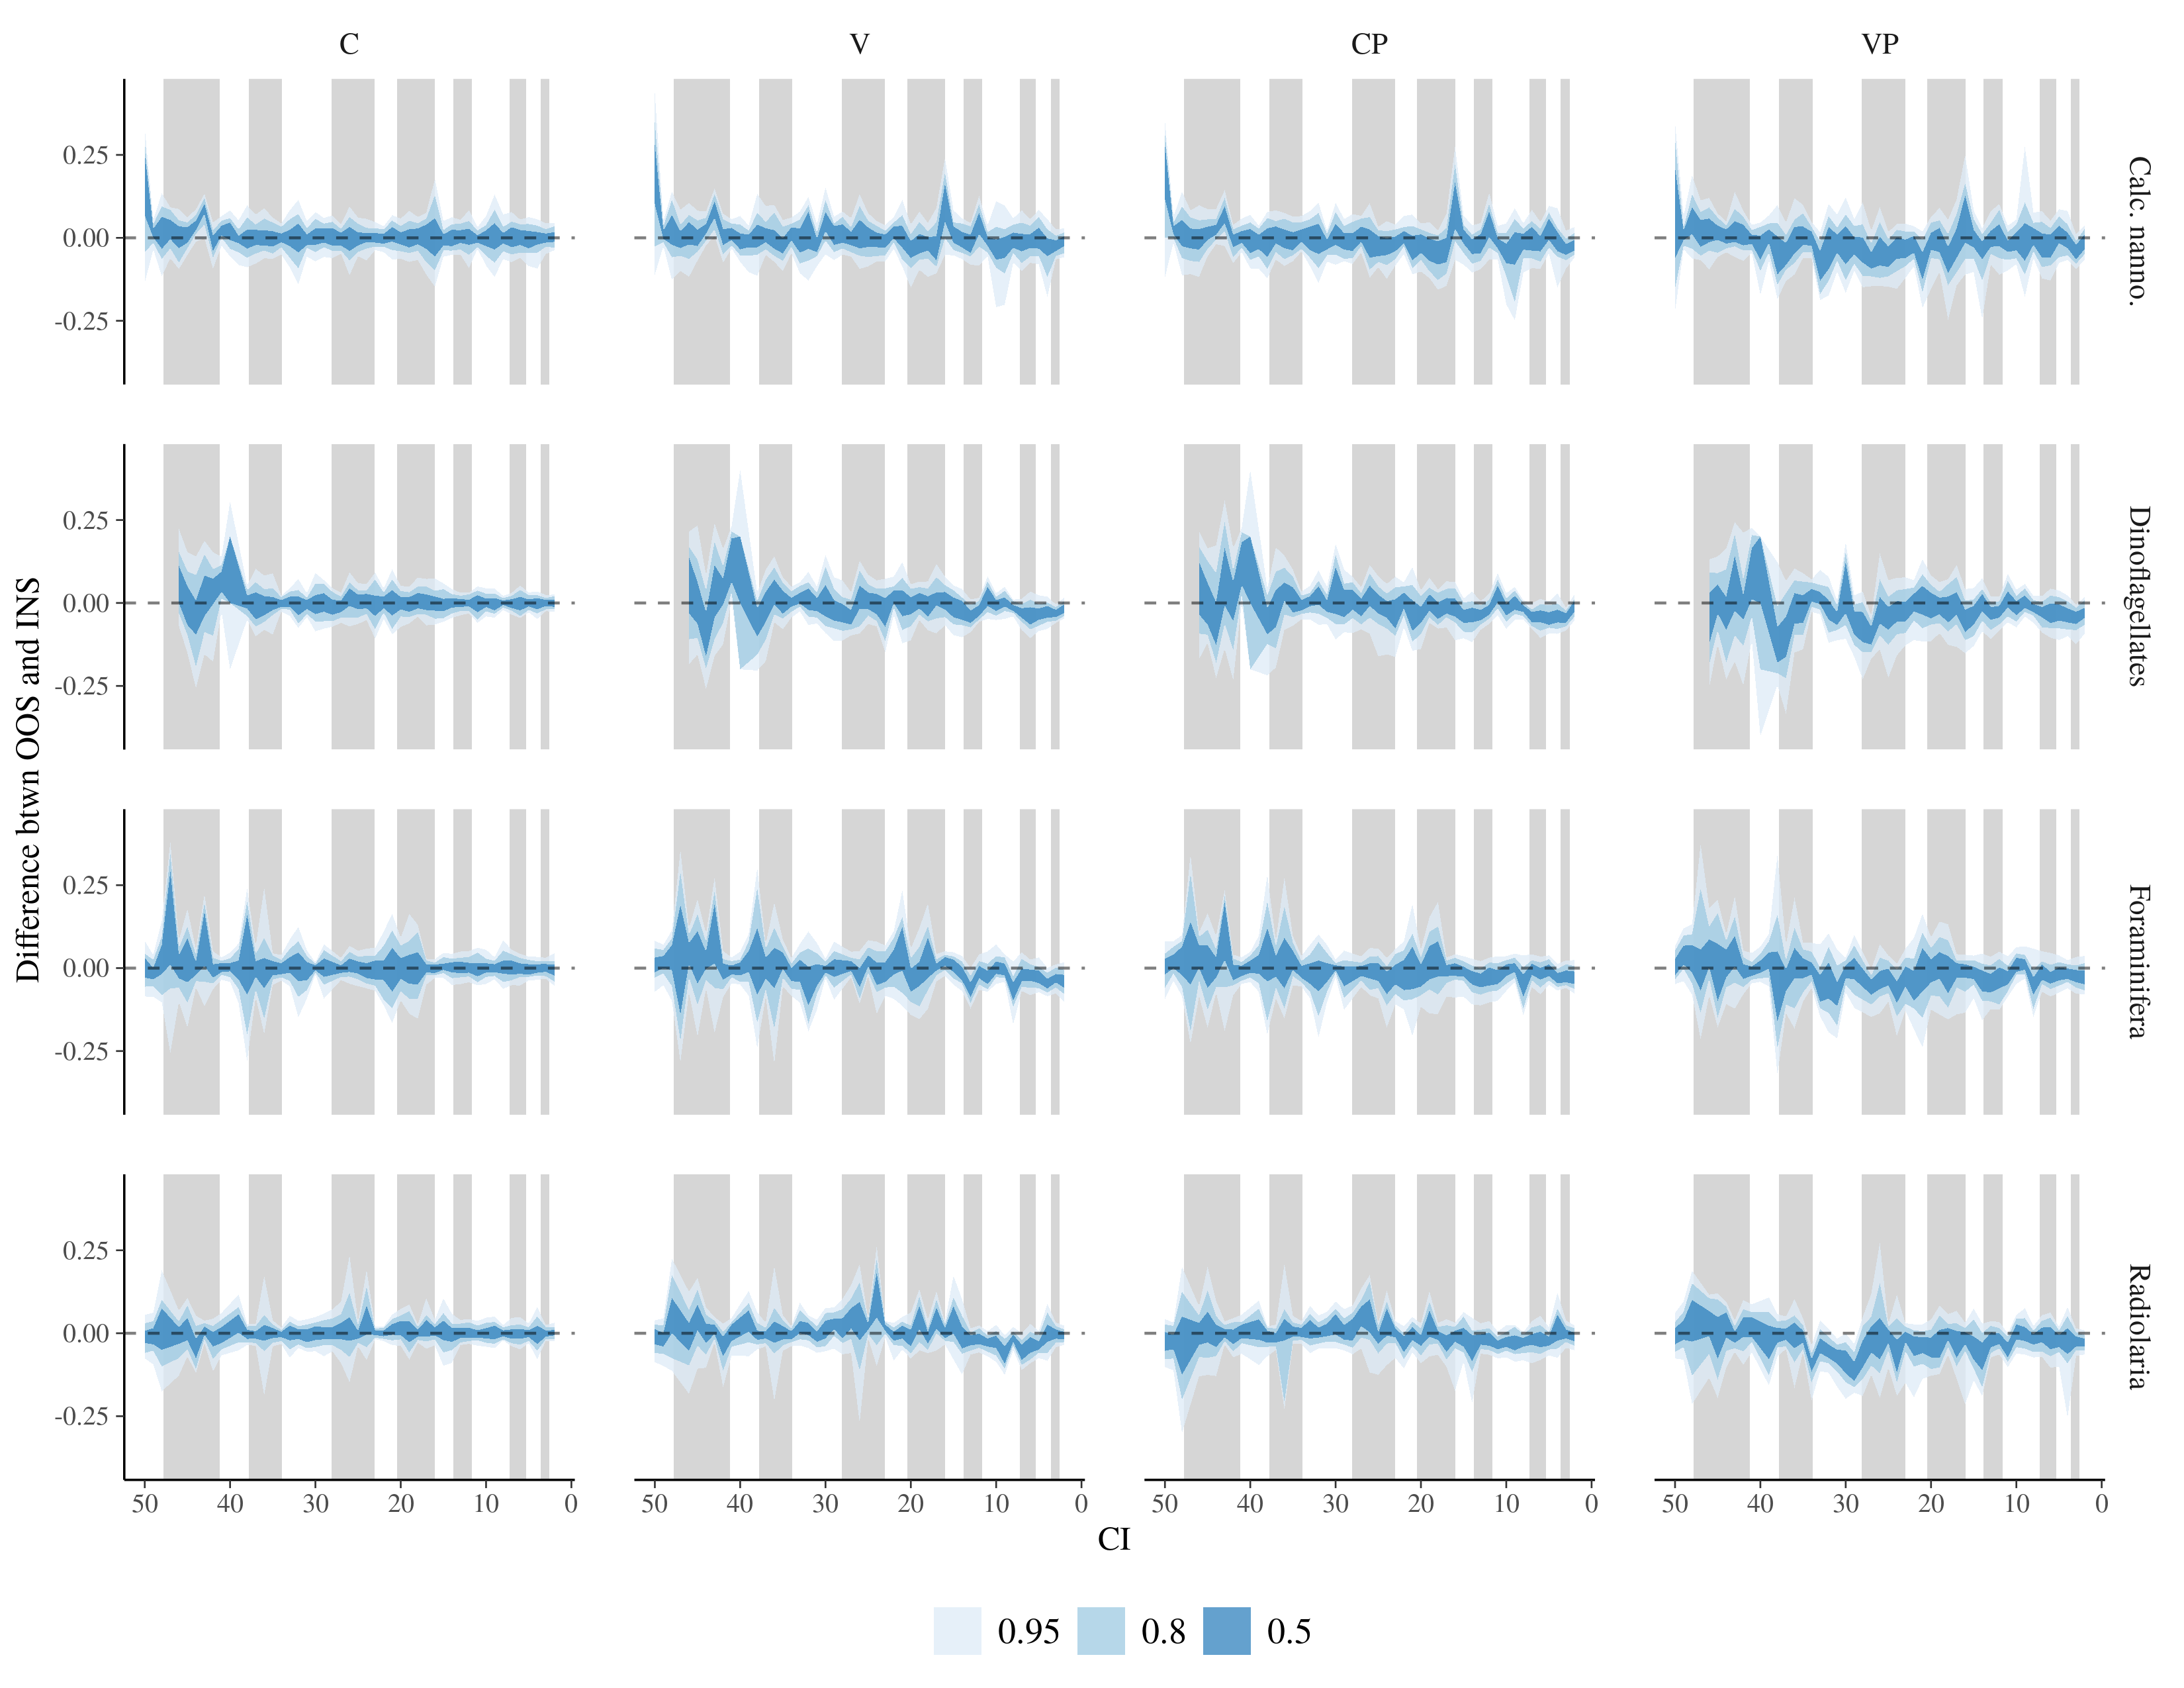
\includegraphics[width=\textwidth,height=0.5\textheight,keepaspectratio=true]{auc_diff.png}
 \caption{Comparing out-of-sample and in-sample forecasts. Congruence between in-sample and out-of-sample indicates that a model is not necessarily overfit to the data. This value is calculated as the values presented in Figure \ref{fig:fold_auc_taxon_time} minus those values presented in Figure \ref{fig:auc_taxon_time}. A differences close to 0 indicate complete congruence between in-sample and out-of-sample forecasts, while a positive difference indicates that the out-of-sample forecasts are actually higher performing than the in-sample forecasts, and a negative difference indicates poorer out-of-sample performance than in-sample forecast. See Table \ref{tab:model_def} for a description of each of the four models (C, V, CP, VP).}
 \label{fig:oos_ins_diff}
\end{figure}




\section{Discussion}

We find that all of our models are expected to correctly forecast which species of randomly selected extinct-extant pair is more likely to go extinct between 70\% to 80\% of the time (Fig. \ref{fig:fold_auc}). These results confirm that past extinction patterns can provide valuable information about which extant species are most threatened with extinction in the near geological future, and that some historical information does not degrade our ability to forecast future extinction risk. To reiterate, all of our models are fit to past extinction events from the Cenozoic and covariates like geographic range or global climate state are associated with these extinctions; our models are conditioned on the past. Some of our models, however, encode historical information such as how covariate effects have varied over time or the change in a species geographic range over time (Table \ref{tab:model_def}). 
%One of the most striking results is that the models that include either the historical covariates (CP model) or allows covariate effects to vary over time (V model) produce less biased out-of-sample forecasts than the model which includes both historical covariates and allows covariate effects to vary over time (VP model) (Fig. \ref{fig:auc_compare}). However, we might expect a potential decrease in precision when forecasting the future of extinction risk is to be expected as the future will always differ from the past in some respect. An extremely important caveat, of course, is that human impacts may substantially alter present and future extinction risk dynamics relative to the average Cenozoic state, so that the future may become less predictable than it has been in the past \citep{Harnik2012a,Finnegan2015}.

Three of the four models we evaluated are practically identical in their ability to make in-sample and out-of-sample forecasts. Although the in-sample AUC estimates differ between models, all of these estimates are in a narrow range of possible AUC values (Fig. \ref{fig:auc_hist}). Our VP model had the best in-sample forecasting results includes the historical covariates and allows all covariate effects to vary over time. However, the out-of-sample forecasts from this model are biased, indicating that it is overfit to the data \ref{fig:fold_auc}). The CP model that includes historical covariates such as geographic range trajectory yields out-of-sample forecasts with nearly identical results to the V model that allows covariate effects to vary over time but does not include historical covariates. 

While all of our models are conditioned on past extinction data from the Cenozoic planktonic microfossil record, we used multiple approaches to encode historical information. Models that include the historical covariates (e.g. change in geographic range) but do not allow covariate effects to vary over time (i.e. CP model) encode the past explicitly but assumes that covariates effects are constant over time. Allowing covariate effects to vary over time, as with our V model, does not explicitly encode the history of individual species into our model but instead models the history of how covariate effects have varied over time, thus implicitly encoding historical information about the species in our models. By modeling the variation in covariate effects over time, forecasts made for future extinction events are conditioned on a wider range of potential covariate effects which can improve our models flexibility when forecasting extinction in the novel environmental conditions we might expect in the future. Comparing our out-of-sample forecast results indicates that these approaches yield approximately equal forecasting performance (Fig. \ref{fig:fold_auc}). Our results contrast somewhat with those of \citet{Kiessling2016}, who found that including historical range trajectories significantly and substantially improved the performance of extinction risk forecasts. Whether this reflects differences in analytical methodology or study system (planktonic microfossil taxa versus marine macroinvertebrates) is not clear and is worth further investigation.

The relative quality and consistency between in-sample and out-of-sample forecasting performance for three of the four models we considered is encouraging given that these estimates are based on very limited biological and environmental information about the studied taxa. Even our most complex models only account for a few simple aspects of geographic range, prior history, and phylogenetic affinity. The principal reason we were not able to include more biological information in the models used here is because we lack additional life history or ecological information for many of the marine micro- and nannoplankton included in this study. Foraminifera are an exception to this problem as aspects of life history, ecology, and physiology are known for many Foraminifera species \citep{Ezard2011}. However, comparable information does not exist for all Foraminifera species, nor does this type of data exist for the other three taxonomic groups studied here. Future analyses including this type of information and focused more narrowly on the Foraminifera may be informative. 

An extremely important caveat, of course, is that human impacts may substantially alter present and future extinction risk dynamics relative to the average Cenozoic state, so that the future may become less predictable than it has been in the past \citep{Harnik2012a,Finnegan2015}. The CP model assumes that the effects of the historical covariates are constant through time, but given growing evidence that human impacts substantially alter extinction risk dynamics \citep{Harnik2012a,Finnegan2015,Payne2007}, this assumption may not be valid and may limit or bias our ability to predict extinction in truly novel environmental regimes. Thus, it might be preferable to use a model similar to our V model which allows extinction risk and selectivity to vary over time. For this reason, while our CP and V models yield similar out-of-sample forecasts, we believe the V model offers more practical benefits for predicting extinction risk in future, anthropogenically impacted environments.

On a related note, it is notable that there are no obvious consistent changes in average model performance during episodes of climatic environmental change such as the mid-Eocene to early Oligocene (Fig. \ref{fig:fold_auc}), although this interval is characterized by elevated extinction among several planktonic groups \citep{Prothero1994,Wade2008,Kamikuri2012}. This suggests that relationships between the simple covariates included in our models and extinction risk were relatively stable though this interval.  However, it is likely that more complex models accounting for other aspects of ecology and biogeography might exhibit reduced forecasting performance during this and other climate change episodes.

To summarize, our results suggest that models trained on prior extinction/survival patterns do modestly well at predicting relative extinction probability of randomly selected species pairs based on a small number of simple taxonomic, geographic, and historical predictors. Although a model that includes historical covariates such as change in geographic range and change in climate between observations while also allowing covariate effects to vary over time performs best at in-sample prediction, this model is overfit to our data and produces less accurate out-of-sample forecasts than our three less complex models. The remaining three models yield nearly equivalent out-of-sample forecasts. The results of this simple exercise suggest that conservation decisions could indeed be bolstered by including fossil data. Additionally, including historical information via explicit modeling of historical covariate effects or modeling how covariate effects have changed over time does not diminish and may ultimately improve our ability to forecast future extinctions. 


\section{Acknowledgements}

We thank Jonathan Payne, Thomas Ezard, Erin Saupe, and Peter Roopnarine for useful discussions. Wolfgang Kiessling, Matthew Clapham, and an anonymous reviewer provided thoughtful reviews that strengthened the manuscript considerably. This work was funded by a David and Lucile Packard Fellowship to SF.


\printbibliography
\end{refsection}
%\clearpage

\end{document}


%\beginsupplement
%\begin{refsection}
%
%\section{Supplemental Figures}
%
%\setcounter{page}{1}
%\section{Supplement to Materials and Methods}
%
%\subsection{Data Specifications} \label{sec:data_desc}
%
%\subsubsection{Binning fossil occurrences}
%
%The estimated age of each occurrence is based on the core-specific age-model that observation is from and can be overly precise. To alleviate this overprecision, we coarsened our temporal information in an effort to limit the effects of between-core heterogeneity in age. The occurrence histories of each species was then summarized as a series of binary codes indicating the presence or last occurrence of that species. For every occurrence of a species, except the last, that species existence and survival is recorded as a 0. The last occurrence of that species is considered the bin in which the taxon has gone extinct -- and is recorded as 1. This protocol means that we are reading the fossil record ``as written,'' a practice that is potentially dangerous as it is an overconfident statement of preservation and may be shortening the actual durations of the studied species \citep{Alroy2010,Alroy2000b,Alroy2014,Foote1997,Foote1999a,Foote2001,Foote1996e,Lloyd2012b,Marshall1995,Wang2016}. However, this practice is common with marine microfossil data due to their exceptional preservation rate \citep{Ezard2013,Ezard2016,Ezard2011,Liow2010}. In fact, with marine microfossils collected from cores a bigger problem may be over extending the duration of a species due to mixing and smearing within the cores \citep{Mekik2018,Broecker1999,Mekik2014,Peng1984}.
%
%
%\subsubsection{Covariate transformation and standardization}
%
%Prior to analysis, geographic range was then log-plus-one transformed and standardized by mean-centering the data and then dividing by the standard deviation of the distribution of geographic ranges. This standardization means that a regression coefficient associated with each covariate describes the change in extinction probability per change in standard deviation of that covariate, that coefficients associated with similarly standardized covariates will be directly comparable in magnitude, and that the intercept term corresponds to the expected value of the outcome at when geographic range is its average value \citep{ARM}. Change in geographic range between observations was measured from the standardized geographic range values and was not standardized separately.
%
%Temperature was also transformed and standardized the in the same manner as geographic range. The change in temperature between an observation and its previous observation was measured from the standardized temperature values and was not standardized separately.
%
%
%\subsection{Model Specifications} \label{sec:model_desc}
%
%In survival analysis, the hazard function describes the instantaneous rate of extinction of a species given its age and covariate information. The hazard function is defined as the conditional probability of a species going extinct by the end of the \(t\)-th interval given that it survived up until \(t\) and the relevant covariate information \(X\) for all \(k\) 1 My intervals \citep{Tutz2016}. For the discrete time intervals \(T = 1, \cdots, k\), extinction is defined as \(T = t\). The discrete time hazard function is defined as
%\begin{equation}
% \lambda(t | X) = P(T = t | T \geq t, X), \quad t = 1, \cdots, k.
% \label{eq:hazard}
%\end{equation}
%
%The hazard function (Eq. \ref{eq:hazard}) is easily reparameterized as a logistic regression by defining that \(\lambda(t | X) = h(\Theta)\) where \(h(.)\) is a logit inverse-link function and \(\Theta\) is the probability of a taxon going extinction during interval \(t\) \citep{Tutz2016}. \(h(\Theta)\) is then modeled as with any regression. In this case, we opted for a hierarchical/mixed-effects model with multiple non-nested varying intercepts and slopes \citep{ARM}.
%
%Our covariates matrix \(X\) is a \(N \times D\) matrix where \(N\) is the total number of observations and \(D\) is the total number of covariates. The first column of \(X\) is entirely 1's as it corresponds to the intercept term in the regression model. The next two columns of \(X\) are two aspects of geographic range as continuous covariates: geographic range \(r\) during interval \(t\), and the difference \(d\) between the geographic range at \(t - 1\) and \(t\). Change in geographic range was calculated from the transformed and standardized geographic range values; this means that change in geographic range is in units of changes in standard deviations. The final two columns are two aspects of global temperature: mean temperature during interval \(t\), and the lag of mean temperature (i.e. mean temperature during interval \(t - 1\).) As with change to geographic range, the lag of temperature is based on the transformed and standardized temperature estimates. 
%
%The matrix of time and phylum varying regression coefficients describing the effects of the covariates on a species' risk of extinction is called \(B\) -- a \(w\) by \(p\) matrix, were \(w\) is the number of time temporal intervals and \(p\) is the number of phyla. The elements of this matrix, the regression coefficients, are themselves modeled as being multivariate normally distributed with vector of means \(\alpha\) describing the average intercept and regression coefficient estimates of each phylum \(p\). These phylum averages are themselves modeled as multivariate normally distributed with mean vector \(\mu\) describing the overall average regression coefficients, including the intercept. \(\mu\) has length \(D\) and is ordered intercept, range coefficient, change in range coefficient, temperature coefficient, temperature lag coefficient.
%
%The effect of species age on the log-odds of species extinction is modeled as a non-nested random intercept \(A\) \citep{Tutz2016}. This term describes how the log-odds of extinction varies along a species duration, and how this effect can differ between the phyla. \(A\) is a \(l\) by \(p\) matrix, where \(l\) is the age at observation of a species and \(p\) is its phylum. \(A\) is modeled as following a multivariate normal distribution with phylum means being the vector \(\delta\) and covariance matrix \(\Sigma_{A}\). The covariation between the elements of vector \(\delta\) are modeled as a multivariate normal distribution with a mean vector of all 0s and covariance matrix \(\Sigma_{\delta}\).
%
%To complete the generative model, we need to assign final priors to the ``top-level'' parameters. In general, we favored weakly informative priors which help regularize our estimates. In the case of a regression coefficient, this means a Normal distribution with mean 0 and a standard deviation of 3. For our scale parameters (e.g. standard deviations), we used half-Cauchy distributed priors with heavy tails but the majority of probability density near 0.
%
%Our top-level intercept was given a more diffuse prior than our regression coefficients, which reflects our greater degree of uncertainty about its value. Our top-level regression coefficient for the effect of geographic range was given an informative prior reflecting the overwhelming amount of evidence that species with a larger than average geographic range have a lower risk of extinction than species with an average or less than average geographic range. In the context of this analysis, this means that we are again using a weakly informative prior but instead of centering the density around -1 (i.e. larger than average geographic range decreases extinction risk).
%
%Instead of assigning a prior distribution for each of the covariance matrices in the model, we instead decomposed the covariance matrices (e.g. \(\Sigma_{B}\)) which allows us to assign independent priors for the scale and correlation aspects of covariance. The scale parameters were assigned half-Cauchy priors as described above in the context of all other scale parameters. The correlation matrices were assigned LKJ priors each with shape parameter set to 1. This choice of shape parameter produces a uniform distribution over possible correlation matrices. These priors are also slightly more interpretable than other common prior distributions for covariance matrices such as the inverse-Wishart distribution. This approach to assigning priors to a covariance matrix is recommended by the Stan Manual \citep{StanManual}.
%
%In total, our model can be expressed as: 
%\begin{equation}
% \begin{aligned}
%  t_{i} &\sim \text{Bernoulli}(\Theta) \\
%  \Theta_{i} &= \text{logit}^{-1} (X_{i} B_{w[i], p[i]} + A_{l[i], p[i]}) \\
%  B_{w, p} &\sim MVN(\alpha_{p}, \Sigma_{B}) \\
%  \alpha_{p} &\sim MVN(\mu, \Sigma_{\alpha}) \\
%  % double check this\dots is A MVN dist?
%  A_{l, p} &\sim MVN(\delta_{p}, \Sigma_{A}) \\
%  \delta_{p} &\sim \mathrm{N}(0, \sigma_{\delta}) \\
%  \mu_{d} &\sim 
%  \begin{cases}
%   N(-2, 5) & \text{if } d = \text{intercept} \\
%   N(-1, 1) & \text{if } d = \text{geo. range} \\
%   N(0, 1) & \text{else } \\
%  \end{cases} \\
%  \delta &\sim N(0, 1) \\
%  \Sigma_{B} &= diag(\tau_{B}) \Omega_{B} diag(\tau_{B}) \\
%  \Sigma_{\alpha} &= diag(\tau_{\alpha}) \Omega_{\alpha} diag(\tau_{\alpha}) \\
%  \Sigma_{A} &= diag(\tau_{A}) \Omega_{A} diag(\tau_{A}) \\
%  \tau_{B} &\sim C^{+}(1) \\
%  \tau_{\alpha} &\sim C^{+}(1) \\
%  \tau_{A} &\sim C^{+}(1) \\
%  \Omega_{B} &\sim LKJ(1) \\
%  \Omega_{\alpha} &\sim LKJ(1) \\
%  \Omega_{A} &\sim LKJ(1) \\
% \end{aligned}
% \label{eq:model}
%\end{equation}
%with \(i\) indexing the observation and bracket subscripts referencing the class of the \(i\)th observation where \(w[i]\) is the time of the \(i\)-th observation, \(p[i]\) is the phylum of the \(i\)-th observation, and \(d[i]\) is the age of the \(i\)-th observation. 
%
%
%\subsection{Model Parameter Estimation} \label{sec:model_est}
%
%We implemented our model (Eq. \ref{eq:model} using the \begin{texttt}rstanarm\end{texttt} package for the R programming language \citep{StanManual}. This package provides an interface to the Stan probabilistic programming language for writing hierarchical/mixed-effects models in native R. Posterior estimates were obtained through Hamiltonian Monte Carlo, using 2000 steps divided equally between warm-up and sampling. In order to prevent divergent transitions adapt delta was increased to 0.999999; all other HMC/NUTS sampling parameters were kept at the defaults for rstanarm 2.18.2 \citep{rstanarm}.
%
%To implement our VP model in \begin{texttt}rstanarm\end{texttt}, where ``data'' is a data.frame object of all necessary data (response, covariates), is coded as:
%\begin{verbatim}
%form <- event ~ 
%        range + range_diff1 + range_diff2 + range_diff3 + 
%        temp + temp_lag + 
%        (1 + range + range_diff + temp + temp_lag | mybin/phylum) + 
%        (1 | age/phylum), 
%stan_glmer(formula = form,
%      data = data, 
%      family = 'binomial',
%      prior = normal(c(-1, 0, 0, 0, 0, 0), rep(1, 6), autoscale = FALSE), 
%      prior_intercept = normal(-2, 5, autoscale = FALSE), 
%      prior_aux = cauchy(0, 1, autoscale = FALSE), 
%      chains = 4,
%      thin = 4,
%      adapt_delta = 0.999999)
%\end{verbatim}
%
%Similarly, our VP model can be implemented using the \begin{texttt}brms\end{texttt} Stan interface \citep{brms2017,brms2018} as:
%\begin{verbatim}
%priors <- c(set_prior('normal(-2, 5)', class= 'Intercept'),
%      set_prior('normal(0, 1)', class = 'b'),
%      set_prior('normal(-1, 1)', class = 'b', coef = 'range'),
%      set_prior('cauchy(0, 1)', class = 'sd'),
%      set_prior('lkj(1)', class = 'cor'))
%form <- bf(event ~ 
%           range + range_diff1 + range_diff2 + range_diff3 + 
%           temp + temp_lag +
%           (1 + range + range_diff + temp + temp_lag | mybin/phylum) +
%           (1 | age/phylum))
%brmfit <- brm(formula = form,
%       data = data, 
%       family = bernoulli(), 
%       prior = priors,
%       chains = 4, 
%       thin = 4,
%       control = list(adapt_delta = 0.999999)
%\end{verbatim}
%
%Posterior convergence was determined using the general and HMC-specific diagnostic criteria: scale reduction factor (\(\hat{R}\); target \(<1.1\)), effective sample size (eff; target value eff/steps \(<0.0001\)), number of samples that saturated the maximum trajectory length for avoiding infinite loops (treedepth; target value 0), sample divergence, and the energy Bayesian Fraction of Mission Information (E-BFMI; target value \(>0.2\)). For further explanation of these diagnostic criteria, see the Stan Manual \citep{StanManual}.
%
%\section{Supplement to Results} \label{sec:supp_res}
%
%Here we present the parameter estimates for our from our VP model (Table \ref{tab:model_def}). We choose to present the estimates from this model because it is our most inclusive model and its parameter estimates are indicative of parameter estimates from other models with a subset of those covariates included in this model.
%
%First, we present the group-level estimates of our regression coefficients and intercept (Fig. \ref{fig:param_est}). Group-level effects are the average effects of that covariate over time and across taxonomic groups. These estimates make up the vector $\mu$ described above. In addition to the average effect of our covariates, we also included the estimate of the group-level intercept, which is the average log-odds of extinction for an average observation over time and across taxonomic groups.
%
%\begin{figure}[ht]
%  \centering
%  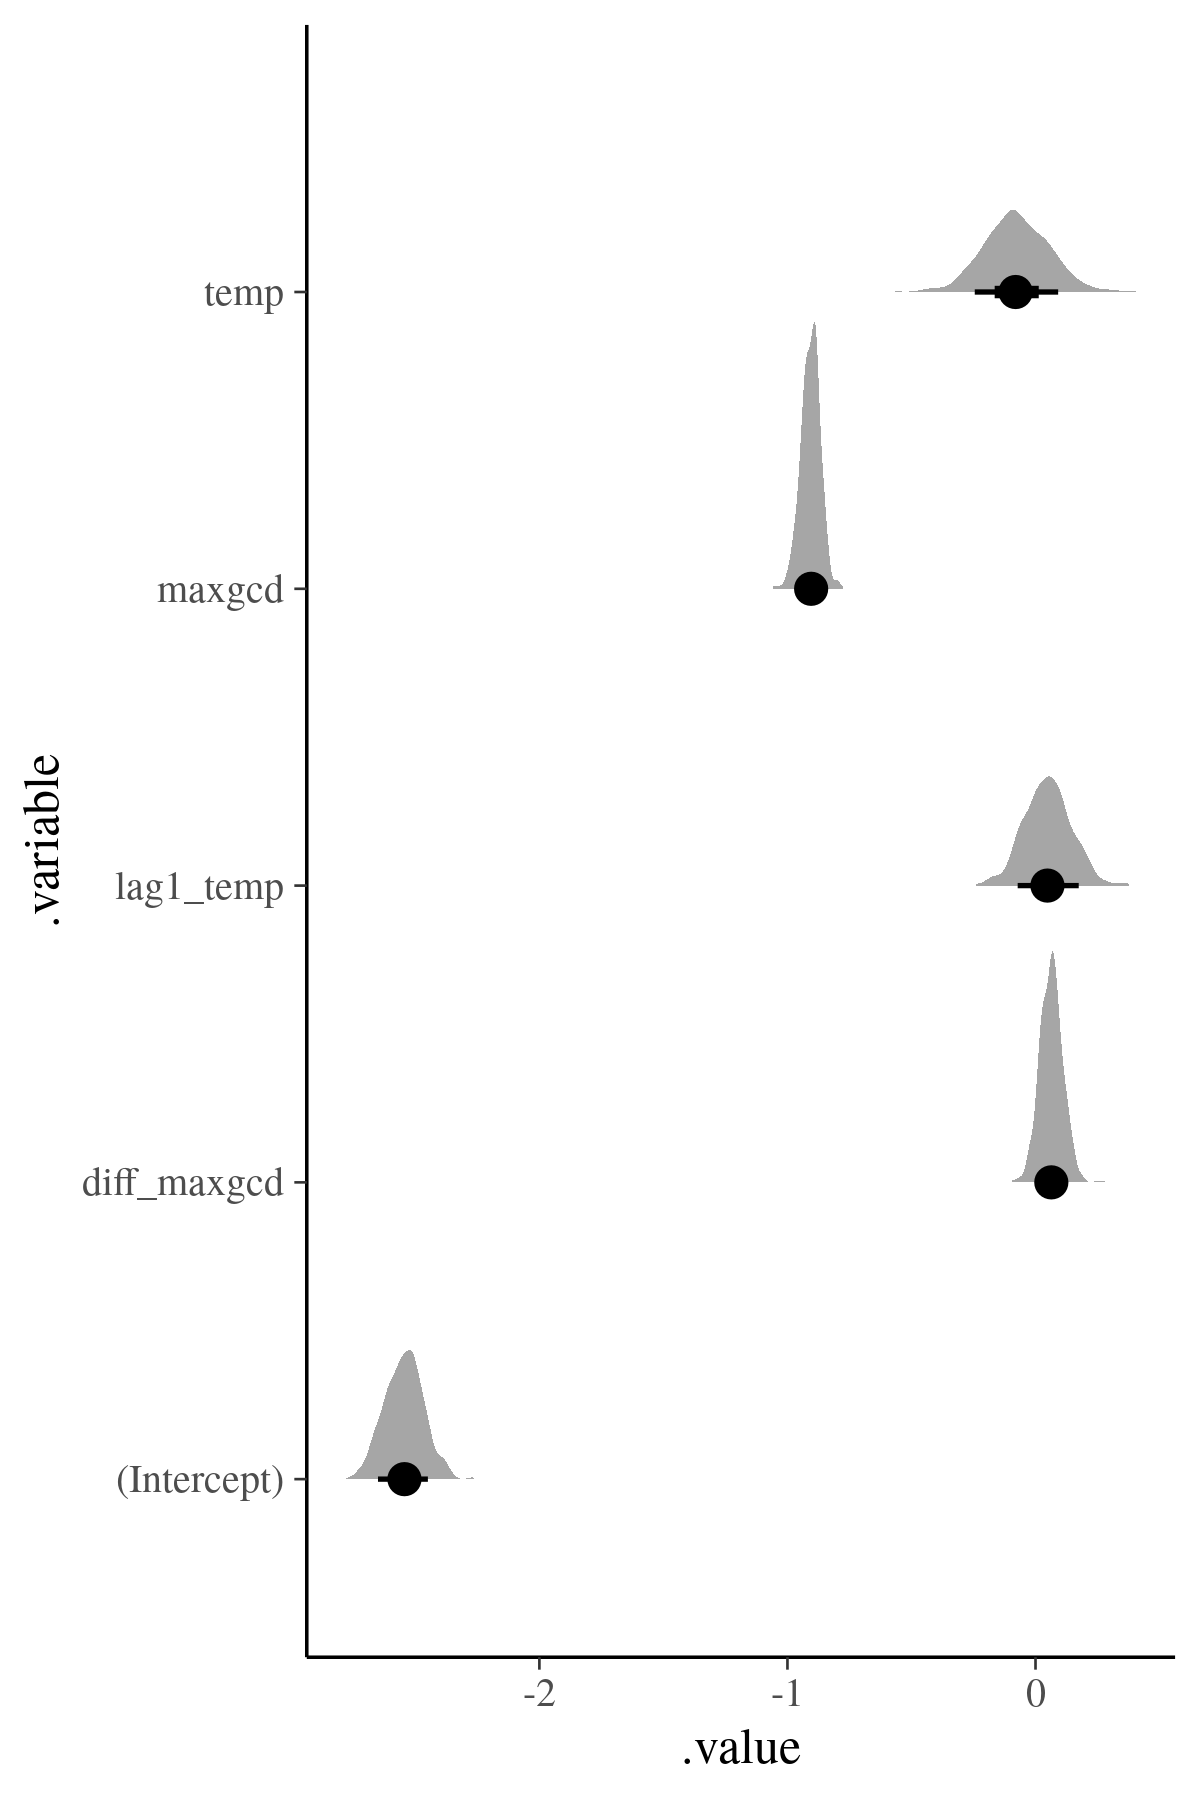
\includegraphics[width=\textwidth,height=\textheight,keepaspectratio=true]{../results/figure/effect_est}
%  \caption{Group-level parameter posterior estimates from our VP model (Table \ref{tab:model_def}). The posterior distribution of our parameter estimates are presented as densities. Below each of these densities is marked the median estimate along with 50\% and 80\% credible intervals. Estimates are on the log-odds scale.}
%  \label{fig:param_est}
%\end{figure}
%
%Second, we present the population-level estimates for our regression coefficients along with the population-level intercept estimates (Fig. \ref{fig:param_est_time_group}. Our VP model allows for these our regression coefficients to vary over time and between taxonomic groups. Population-level estimates are those for a specific time interval and taxonomic group. In this case, the intercept estimate describes the log-odds of extinction for an average observation at that point in time and taxonomic group.
%
%\begin{figure}[ht]
%  \centering
%  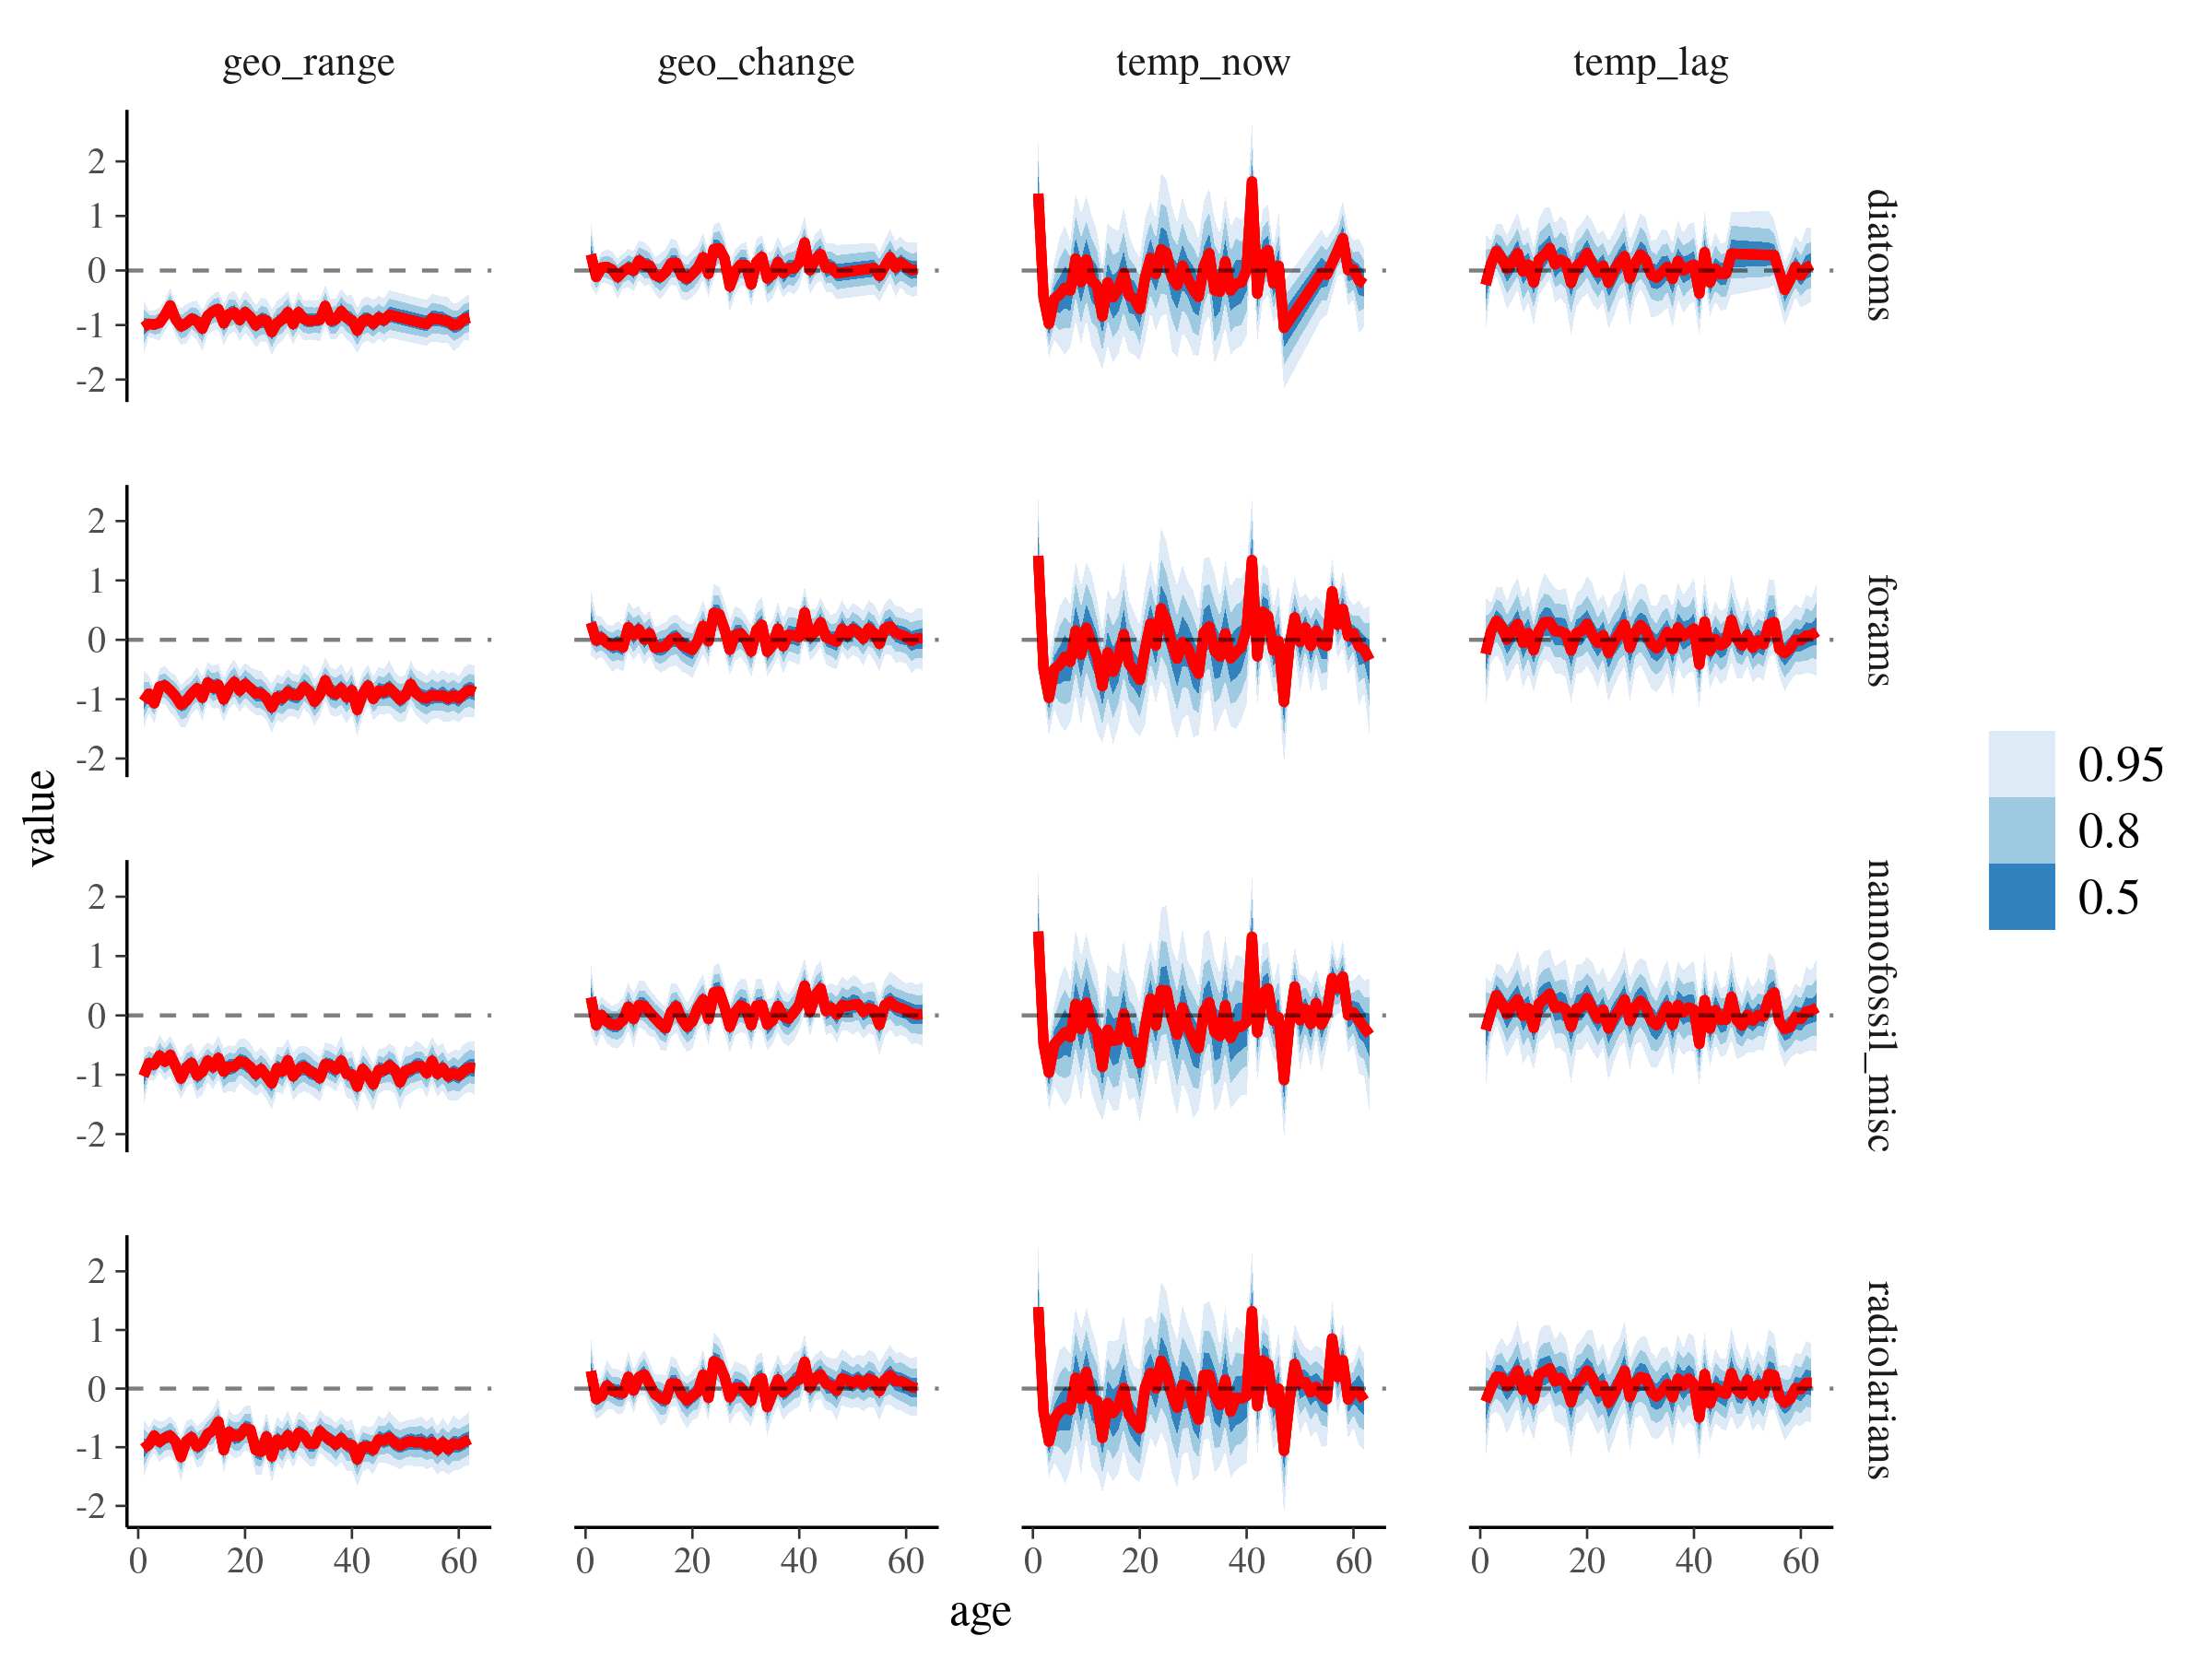
\includegraphics[width=\textwidth,height=\textheight,keepaspectratio=true]{../results/figure/eff_time_group}
%  \caption{Population-level parameter posterior estimates from our VP model (Table \ref{tab:model_def}). Posterior estimates are presented as a time series. The black line represents the median estimate of that parameter. In addition, the 50\%, 80\%, and 95\% credible intervals are indicated. Estimates are on the log-odds scale.}
%  \label{fig:param_est_time_group}
%\end{figure}
%
%
%
%\printbibliography[title={Supplementary References}]
%\end{refsection}

